
\documentclass[twocolumn]{article}
\usepackage{mathpazo}
\usepackage{microtype}
\usepackage{times}
\usepackage{titlesec} % 1
\usepackage[colorlinks = true,
            linkcolor = blue,
            urlcolor  = blue,
            citecolor = blue,
            anchorcolor = blue]{hyperref}
%\usepackage{sectsty} % "제 1 절" ...

 %%%%%%%%%%%%%%%%%%%%%%%%%%%%%%%%%%%%%%%%%%%%%%%%%%%%%%%%%%%%%%%%%%%%%%%%%%%%%
 %                              My Commands
\newcommand{\bi}{\begin{itemize}}
\newcommand{\ei}{\end{itemize}}
\newcommand{\be}{\begin{enumerate}}
\newcommand{\ee}{\end{enumerate}}
\newcommand{\ii}{\item}
\newtheorem{Def}{Definition}
\newtheorem{Lem}{Lemma}
\usepackage{algorithm}
\usepackage{algorithmicx}
\usepackage{algpseudocode}

\usepackage{graphicx}
\graphicspath{%
        {converted_graphics/}
        {./images/}
}

\usepackage{color}
\usepackage{xcolor}
\usepackage{listings}
\usepackage{caption}
\DeclareCaptionFont{white}{\color{white}}
\DeclareCaptionFormat{listing}{\colorbox{gray}{\parbox{\textwidth}{#1#2#3}}}
\captionsetup[lstlisting]{format=listing,labelfont=white,textfont=white}
\usepackage{verbatimbox}

\usepackage[hangul,nonfrench,finemath]{kotex}
    
\setlength\textwidth{7in} 
\setlength\textheight{9.5in} 
\setlength\oddsidemargin{-0.25in} 
\setlength\topmargin{-0.25in} 
\setlength\headheight{0in} 
\setlength\headsep{0in} 
%\setlength\columnsep{5pt}
\sloppy 
 
\begin{document}

\title{
\vspace{-0.5in}\rule{\textwidth}{2pt}
\begin{tabular}{ll}\begin{minipage}{4.75in}\vspace{6px}
\noindent\large {\it KIWI Project}@Data Management Research Section\\
\vspace{-12px}\\
\noindent\LARGE ETRI\qquad  \large Technical Report 15ZS1410-TR-75
\end{minipage}&\begin{minipage}{2in}\vspace{6px}\small
218 Gajeong-ro, Yuseong-gu\\
Daejeon, 305-700, South Korea\\
http:/$\!$/www.etri.re.kr/\\
http:/$\!$/sungsoo.github.com/\quad 
\end{minipage}\end{tabular}
\rule{\textwidth}{2pt}\vspace{0.25in}
\LARGE \bf 국외 출장 보고서 \\
\large The 2015 International Conference on High Performance Computing \& Simulation (HPCS 2015)
}

\date{}

\author{
{\bf 김성수 (Sung-Soo Kim)}\\
\it{sungsoo@etri.re.kr}
}

\maketitle

\begin{abstract}
고성능 컴퓨팅(High-Performance Computing, HPC)은 고급 연산 문제를 풀기 위하여 슈퍼컴퓨터 및 컴퓨터 클러스터를 사용하는 것을 말한다. 
고성능 컴퓨팅 기술은 빅 데이터 분석 플랫폼을 개발하기 위해서 필요한 핵심 요소기술 중 하나다. 
금번 13번째 HPCS 2015 학회는 네델란드 암스테르담 힐튼 호텔에서 열렸다. 
출장자는 논문 발표 및 빅데이터 분산 병렬처리 관련 최신 연구동향 파악을 목적으로 학회에 참석하였다.
금번 학회 논문 채택률은 37\%로 45편의 full paper가  채택되었고, 6개 관련워크샵 참석자들을 합쳐 180여명이 참석하였다.
다음번 학회 HPCS 2016은 오스트리아 빈에서 개최될 예정이다.

본 출장보고서는 HPCS 2015에서 참석했던 튜토리얼 및 세션을 중심으로 연구 동향을 살펴보고, 또한 해당 주제와 관련된 가트너 (Gartner) 자료를 조사하여 함께 정리함으로써, 연구동향 파악에 도움이 될 수 있는 기술문서 형태로 작성하였다. 본 출장보고서가 현재 연구분야 수행 및 신규 프로젝트 기획 시 도움이 되길 진심으로 바란다.
\end{abstract}

\section{서론}
과학 연구와 연관된 고성능 컴퓨터의 이용을 일반적으로 널리 쓰이는 고성능 컴퓨팅의 정의로 본다. 
고성능 컴퓨팅(High Performance Computing, HPC)이라는 분야는 지난 수십년 동안의 IT 기술 발전의 선도 역할을 수행해 왔음에 틀림이 없다. 

HPC 기술 발전의 결과물로 고성능 멀티 코어 프로세스, 저전력 서버 기술, 인피니밴드와 같은 고성능 네트워크 기술, 대용량 저장을 위한 스토리지 시스템 기술 등이 현실화되었으며, 이는 HPC 분야 뿐만 아니라 클라우드로 통칭되는 현대의 모든 IT 기술의 기반이 되었다고 해도 과장이 아니다.

이번 HPCS 2015 학회 참석을 통해, 이러한 HPC, 클라우드, 빅데이터를 모두 포괄하는\textit{ e-Science}, 즉, 데이터 집약적 과학적 발견 (data-intensive scientific discovery)과 관련된 주요 연구 결과를 살펴 볼 수 있었으며, 필자에게는 진행하고 있는 과제와 관련된 최신 연구동향을 배울 수 있었던 아주 유익한 출장이었다. 
또한, 연구결과에 대한 논문발표 뿐만 아니라, 국제학회에서 세션 좌장 (session chair) 역할을 수행함으로써, 학회에 기여하면서 개인적으로는 좋은 경험을 쌓을 수 있었다.
필자가 금번 출장을 통해 배우게 된 핵심 내용을 키워드로 요약 정리하면 아래와 같다.

\bi
\ii Large Scale Distributed Computing
\ii Science Gateways
\ii Accelerated Cloud
\ii Software-Defined [\textit{Everything}]
\ei
\subsection{출장 개요}

\bi
\ii 출장자: 김성수 선임연구원 (데이터관리연구실)
\ii 출장목적: HPCS 2015 논문발표 및 빅데이터 분산 병렬처리 관련 최신 연구동향 파악
\ii 출장기간: 2015.07.19 - 2015.07.26 (6박 8일)
\ii 장소: 암스테르담 힐튼호텔 (네델란드)
\ii 수행과제: 배치/온라인 듀얼 모드 빅데이터 분석 플랫폼 기술 개발 [15ZS1410]
\ei

\subsection{출장 세부 일정}

\begin{tabular}{ c | c } 
\hline	
\textbf{일자} & \textbf{주요 활동 내용} \\ 
\hline 
\hline
2015.07.19 & 대전 출발, 암스테르담 도착 \\ 
2015.07.20 - 2015.07.24 & 학회 등록 및 논문 발표 (7/22)  \\ 
 					 & 튜토리얼 세션 및 논문 세션 참석 \\ 
2015.07.25 - 2015.07.26 & 암스테르담 출발, 대전 도착 \\
\hline 
\end{tabular}



\section{참석 세션}
본 출장보고서에서 참석한 세션별 각 발표 내용에 대해 아래와 같은 형식으로 정리하고자 한다.
\bi
\ii \textbf{Contributions:} 발표의 주요한 연구 기여에 대해 기술
\ii \textbf{Why:} 왜? 발표 주제가 중요한가? 흥미로운가? 
\ii \textbf{How:} 연구목표를 달성하기 위해 어떠한 접근법(방법)을 적용했는가 기술
\ii \textbf{What:} 연구 수행결과로 도출된 주요 결과물 기술
\ii \textbf{Technology Trends:} 연구 주제와 관련된 가트너 (Garnet) 자료와 연관된 분석내용을 기술
\ei

\subsection{Tutorials}
튜토리얼은 학회 첫날(7/20) 총 5개의 주제에 대해 병렬 세션으로 진행되었으며, 3개의 튜토리얼에 참석하였다.
첫번째 튜토리얼은 대규모 분산환경에서 다양한 워크로드를 실행할 수 있는 오픈소스 워크로드 엔진인 OpenMOLE에 대해 4시간 발표가 있었다.
이후 Science Gateways 주제로 2시간 튜토리얼이 진행되었다. 세번째 참석 세션은 인텔 멀티코어 CPU에 있는 벡터처리용 보조 프로세스를 활용한 벡터화(vectorization) 프로그래밍에 대한 주제로 세시간 반의 튜토리얼에 참석했다.

\subsubsection{Model Exploration using OpenMOLE: A Workflow Engine for Large Scale Distributed Design of Experiments and Parameter Tuning}
\textbf{Speakers:} Romain Reuillon$^1$, Mathieu Leclaire, Jonathan Passerat- Palmbach$^2$, $^1$Complex Systems Institute, Paris, France; $^2$BioMedIA Group, Imperial College London, London, U.K.

OpenMOLE (Open MOdeL Experiment)은 분산 컴퓨팅 환경에서 프로그램 실행을 간단하게 수행할 수 있게 해 준다 \cite{openmole:2015}. 3명의 발표자가 튜토리얼을 7월 20일 오전 4시간에 걸쳐 마치 토론하듯이 진행했다.
OpenMOLE은 다양한 입력 (매개 변수 또는 데이터 세트)에 대해 동일한 프로그램을 실행하려면 필요한 도구다. 
OpenMOLE의 일반적인 유즈케이스로는 고성능 모델 정합 (high performance model calibration), 모델 탐사 (model exploration), 기계 학습 (machine learning), 최적화, 데이터 처리가 있다. OpenMOLE은 다음과 같은 특징을 제공한다.
\bi
\ii \textbf{Works with your programs} - Java, Binary exe, NetLogo, R, SciLab, Python, C++...
\ii \textbf{Distributed computing} - Works on your multi-core machines, clusters, grids, desktop grid.
\ii \textbf{Expressive} - Graphical and scripted workflow system to describe your naturally parallel processes.
\ii \textbf{Scalable} - Handles millions of tasks, years of computation, and GBs of data.
\ii \textbf{Mature} - Developed since 2008 and widely used.
\ii \textbf{Open} - AGPLv3 free software license.
\ei

\begin{figure}[htb]
        \centering
        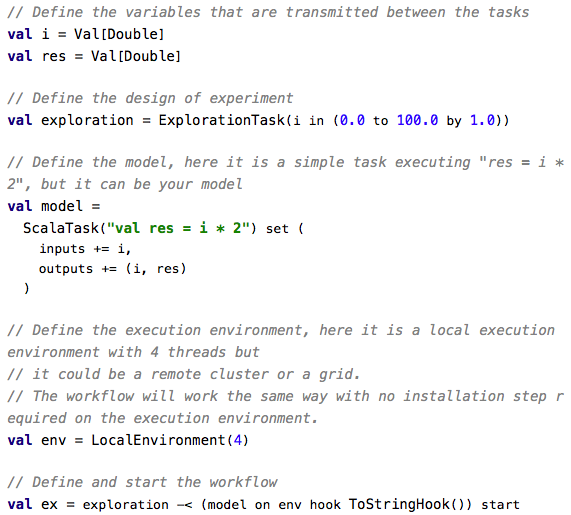
\includegraphics[width=0.49\textwidth]{openmole-code.png}
        \caption{An OpenMOLE Hello World!}
        \label{fig:openmole-code}
\end{figure}

\noindent
\textbf{Contributions:} OpenMOLE은 분산 컴퓨팅 환경에서 다양한 워크로드 실행시 파라미터를 조절해가며 실행할 수 있는 워크로드 실행 엔진이다. 
사용자는 간단한 DSL (Domain-Specific Language)를 이용하여 실행 로직을 코드로 기술함으로 간단히 분산 컴퓨팅 환경 실행을 수행할 수 있다.

\noindent
\textbf{Why:} 다양한 분산 컴퓨팅 환경과 세부 응용 소프트웨어에 대한 파라미터 조절을 해 가며 워크로드를 실행하기 위해서는 워크로드 실행 엔진이 필요하다.

\noindent
\textbf{How:} OpenMOLE은 사용자가 지정한 워크로드를 실행할 수 있는 플랫폼(워크로드 실행엔진)과 도메인 전용 언어(DSL; Domain-Specific Language)를 제공한다.

\noindent
\textbf{What:} OpenMOLE은 오픈소스 프로젝트로 진행 중이며, 관련 프로젝트 웹사이트 (http://next.openmole.org)에 가면 소스 코드 및 실행가이드를 제공받을 수 있다. 그림 \ref{fig:openmole-code}은 OpenMOLE DSL를 이용한 매번 수행시 2씩 곱하는 간단한 응용프로그램이다. 이 계산은 로컬머신에서 멀티 쓰레드 환경에서 실행된다.

또 다른 실습으로 Monte-Carlo Pi estimation 예제와 Random Forest 예제 프로그램을 OpenMOLE에서 실행하는 실습도 함께 진행했다. 실습은 OpenMOLE 프로젝트 사이트 \cite{openmole:2015}에서 필요한 파일을 다운받아 설치 후, command line 또는 웹 GUI를 통해 비교적 쉽게 실습해 볼 수 있다.

\noindent
\textbf{Note}: \textit{Random Forests, Bagging and Boosting} --
"Random forests are an ensemble learning method for classification (and regression) that operate by constructing a multitude of decision trees at training time and outputting the class that is the mode of the classes output by individual trees." — "Random Forest," Wikipedia, 3 November 2014.

\subsubsection{Science Gateways – Leveraging Modeling and Simulations in HPC Infrastructures via Increased Usability}
\textbf{Speakers:} Sandra Gesing, University of Notre Dame, Indiana, USA


\subsubsection{Getting Started with the AVX-512 on the Multicore and Manycore Platforms}
\textbf{Speakers:} \\
Elmoustapha Ould-ahmed-Vall, Intel Corporation, Phoenix, Arizona, USA\\ 
Shuo Li, Intel Corporation, Portland, Oregon, USA\\
Bob Valentine, Intel Corporation, Haifa, Israel\\
Jesus Corbal, Intel Corporation, Barcelona, Spain

고급 벡터 확장(Advanced Vector Extensions,약어:AVX)은 2008년 4월 춘계 인텔 개발자 포럼에서 발표된 x86 명령어 집합의 확장으로 SIMD명령어 집합중의 하나이다. SIMD 레지스터의 폭이 128비트에서 256비트로 확장돼서, 최대 2배까지 부동소수점 연산 처리 능력이 향상된다. 또한 기존의 2 피연산자 구조에서 3 피연산자 구조로 변경됨으로 인하여 프로그래밍이 더 효율적이고 성능이 더 뛰어나게 된다. 

\begin{figure}[htb]
        \centering
        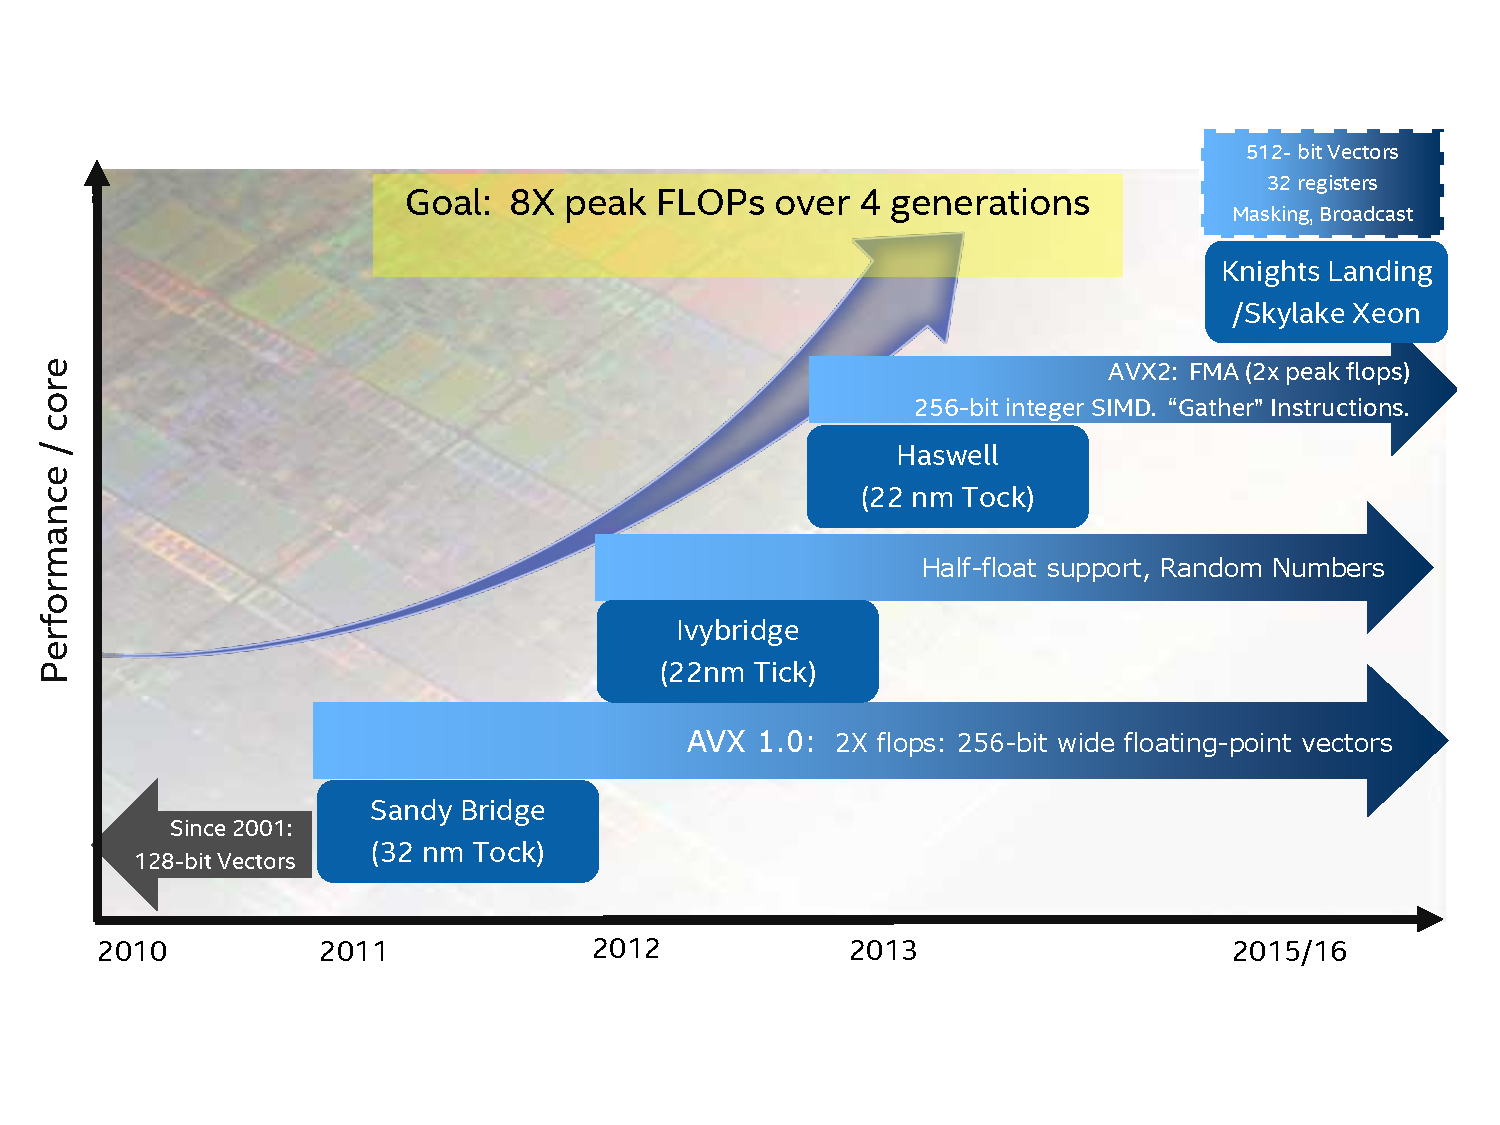
\includegraphics[width=0.48\textwidth]{intel-avx.pdf}
        \caption{Intel Advanced Vector Extensions}
        \label{fig:intel-avx}
\end{figure}

\noindent
\textbf{Contributions:} 그림 \ref{fig:intel-avx}는 Intel Advanced Vector Extensions (Intel AVX)에 대한 로드맵을 보여주고 있다.
향후 Intel의 새로운 제품은 512 비트 SIMD 지원할 예정이다. 이 제품은 단일 명령어 IntelAVX / AVX2 대비 두 배의 처리, 인텔 SSE 성능에 비해 4 배 성능 개선을 가능하게 한다. 특히, 빅데이터 분석에서 데이터레벨 병렬성 (data-level parallelism)을 갖는 문제에 대해 처리속도 개선에 큰 도움이 되리라 기대한다. 출시 예정인 AVX-512에 대한 세부 명령어 및 기능을 배울 수 있었던 유익한 튜토리얼이였다.

\begin{figure}[htb]
        \centering
        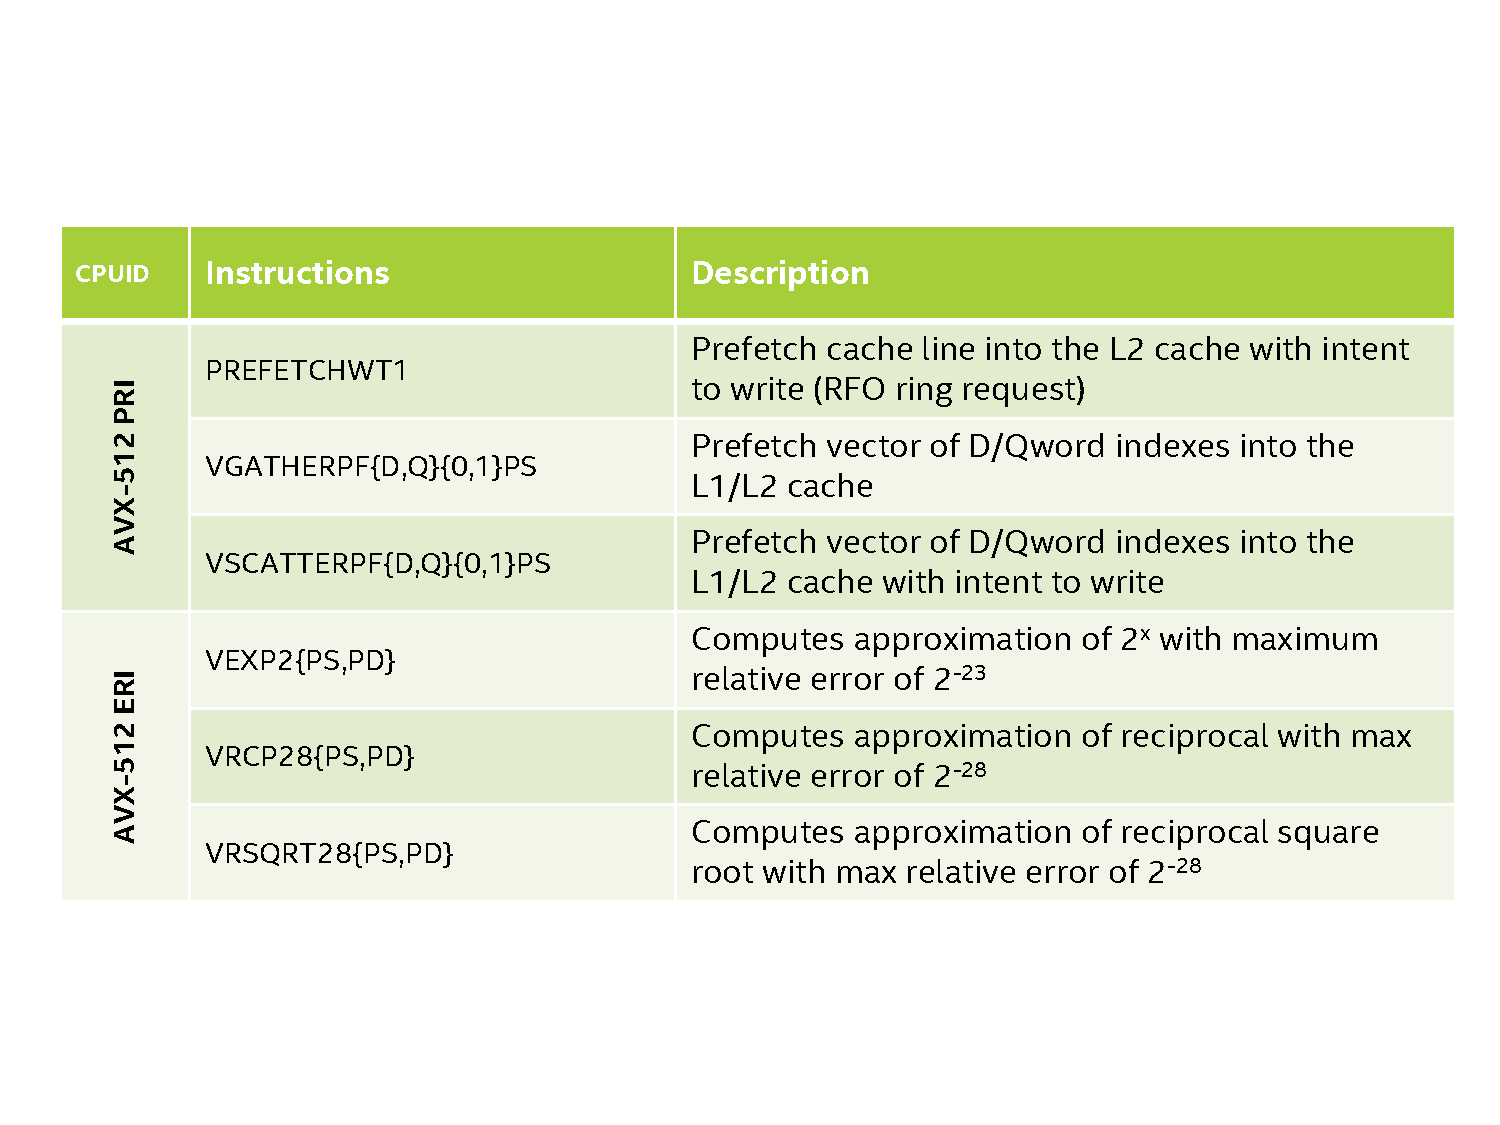
\includegraphics[width=0.48\textwidth]{intel-table.pdf}
        \caption{AVX-512 ERI \& PRI Description}
        \label{fig:intel-avx-description}
\end{figure}

그림 \ref{fig:intel-avx-description}은 Intel AVX-512 Exponential and Reciprocal Instructions (ERI) 명령어를 보여주고 있다. 그림 \ref{fig:intel-avx-512}는 ERI 및 PRI 명령어의 제공 동기 (motivation)를 보여주고 있다.

\noindent
\textbf{Why:} 
인텔 AVX-512는 대부분 요구되는 계산중심 작업시에 고성능을 제공하기 때문에 중요하다.

\begin{figure}[htb]
        \centering
        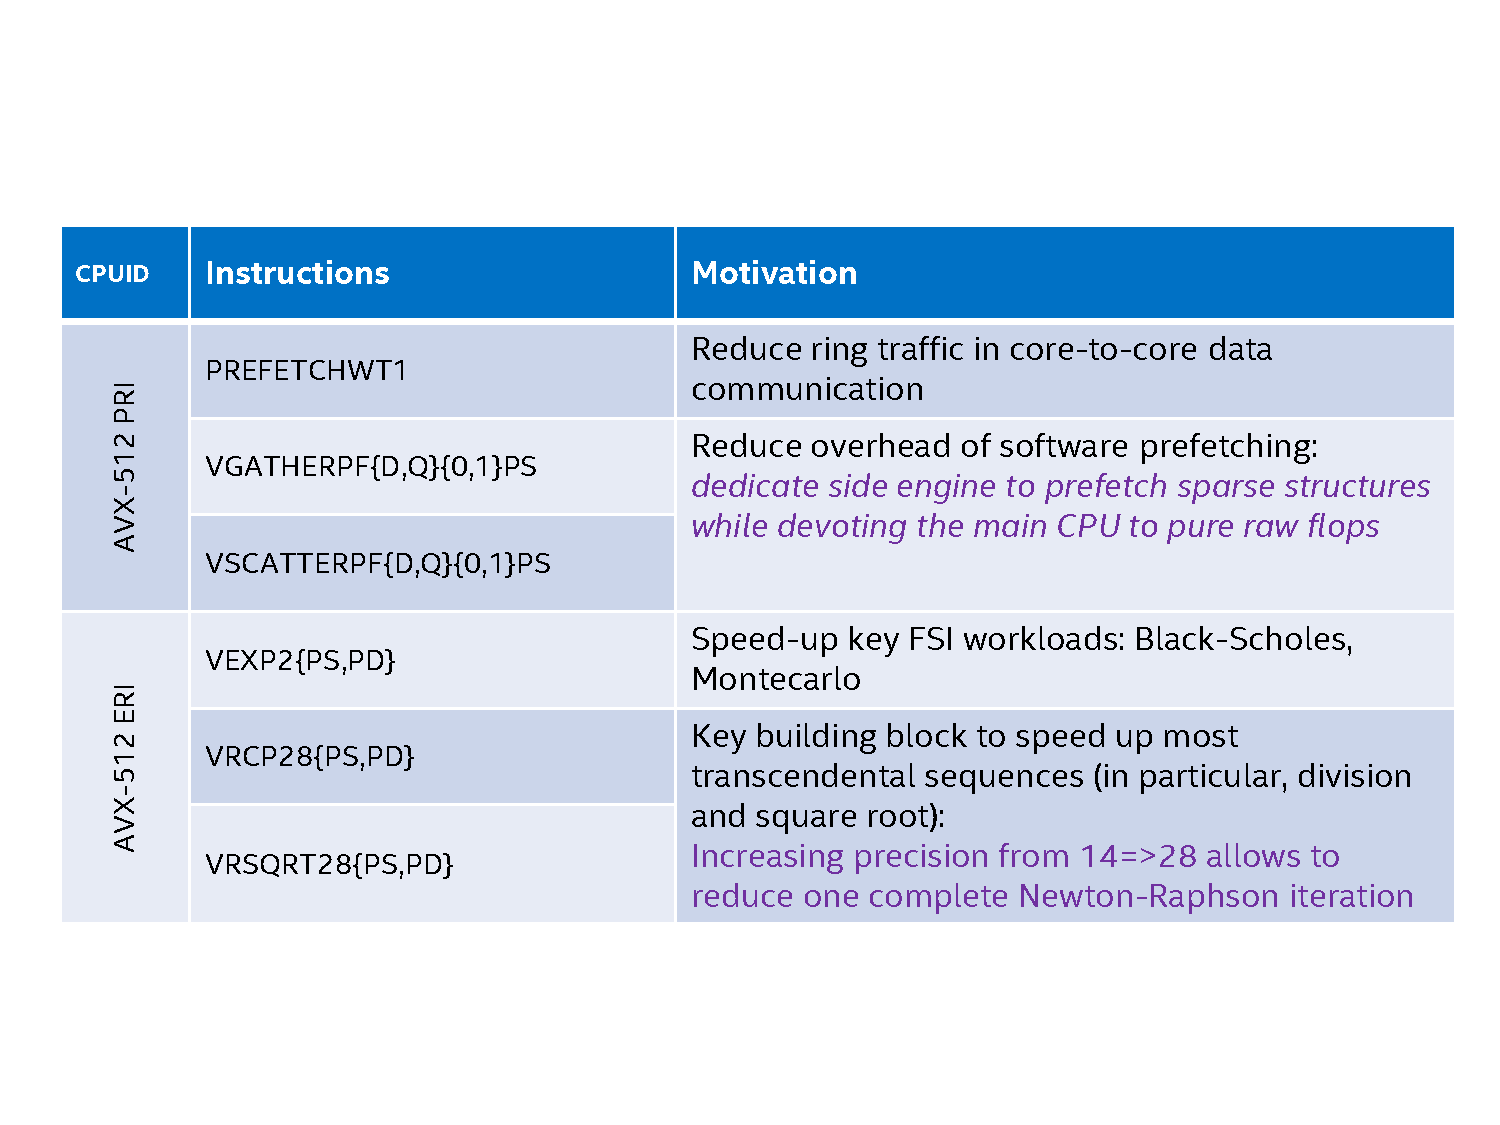
\includegraphics[width=0.48\textwidth]{intel-avx-512.pdf}
        \caption{AVX-512 ERI \& PRI Motivation}
        \label{fig:intel-avx-512}
\end{figure}

\noindent
\textbf{How:} 인텔 AVX-512 명령어는 명령 기능의 설계에서 전례없는 처리 성능과 최고 수준의 컴파일러 지원을 제공한다.

\noindent
\textbf{Note:} \textit{Intel AVX-512 features} include 32 vector registers each 512-bit wide and eight dedicated mask registers. Intel AVX-512 is a flexible instruction set that includes support for broadcast, embedded masking to enable predication, embedded floating point rounding control, embedded floating-point fault suppression, scatter instructions, high speed math instructions, and compact representation of large displacement values.

\noindent
\textbf{What:} CPUID에 따라 인텔 AVX-512 ERI 및 PRI 명령어를 제공한다.

\subsection{Keynote Presentation}
슈퍼컴퓨팅 변화에 대한 소프트웨어 변화전략, GPU 기반 클라우드 가속화 기술, e-Science를 위한 복합 e-Infrastructure, 유럽지역의 컴퓨팅 인프라 및 로드맵인  EGI-Engage등 4개 주제로 키노트 발표가 있었다. 본 절에서는 슈퍼컴퓨팅 변화에 대한 소프트웨어 변화전략과 GPU 기반 클라우드 가속화 기술에 대한 키노트 발표에 대해 기술한다.

\subsubsection{Architecture-aware Algorithms and Software for Peta and Exascale Computing}
\textbf{Speaker:} Jack Dongarra\\
University of Tennessee and Oak Ridge National Lab, Tennessee, USA; University of Manchester, U.K.

\noindent
\textbf{Contributions:} 본 키노트 발표에서는 지난 10년 동안 고성능 컴퓨팅 기술 변화에 대해 살펴보고, 주요 기술 동향에 따른 미래 예상되는 HPC 기술들에 대해 설명해 주었다. 그림 \ref{fig:hpc_20}은 지난 20년간 HPC 성능개발 변화 추이를 그래프이다. 현재 아이폰은 20년전 슈퍼컴퓨터의 성능과 동일함을 알 수 있다. 하지만, 발표자는 이러한 하드웨어 성능 개선속도에 비해 소프트웨어 변화가 더딘면이 있다고 지적했다.

\begin{figure}[htb]
        \centering
        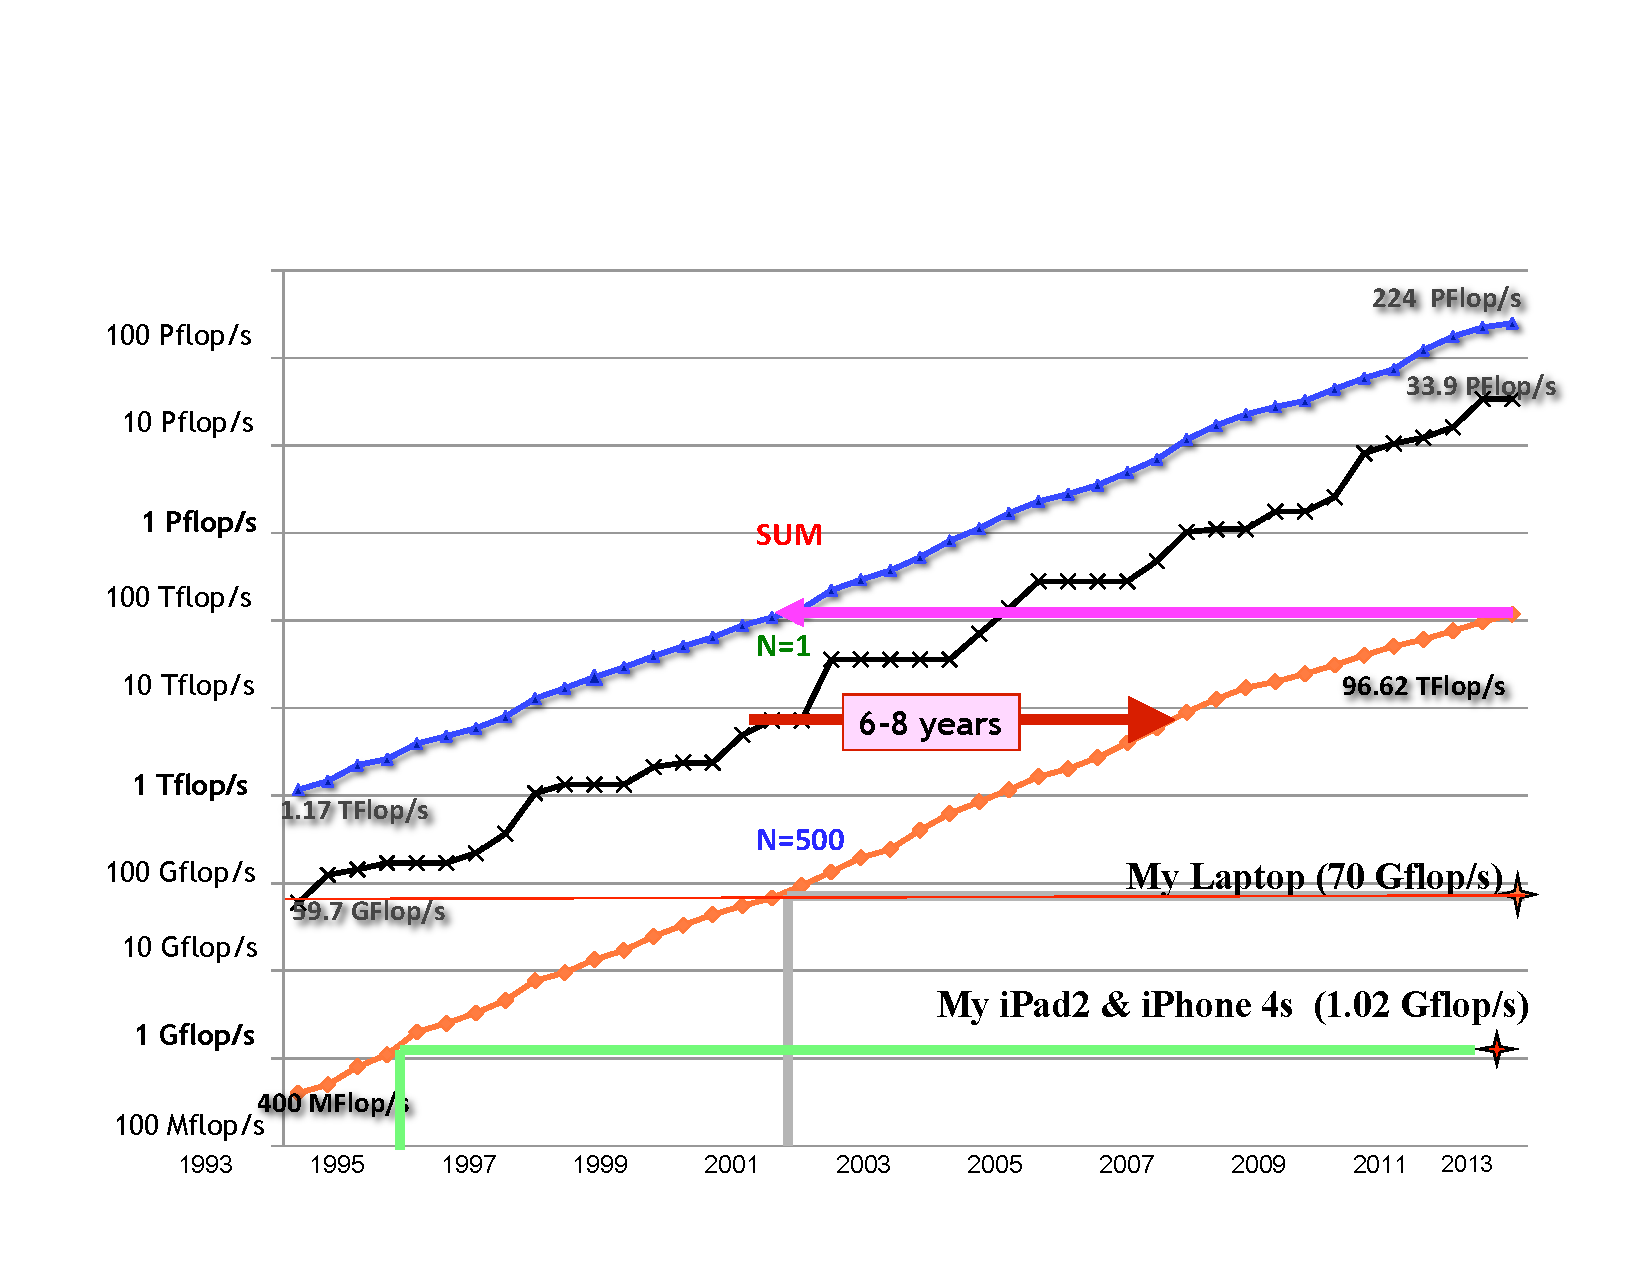
\includegraphics[width=0.48\textwidth]{hpc-20-years.pdf}
        \caption{Performance development of HPC over the last 20 years.}
        \label{fig:hpc_20}
\end{figure}
\noindent
\textbf{Why:}  지난 20년간 HPC 분야는 하드웨어 측면만을 지나치게 강조해서 연구개발 투자가 이루어져 왔다. HPC 기술 및 패러다임 변화는 우리가 개발하는 소프트웨어에 큰 영향을 미치기 때문에, HPC 기술이 어떻게 진화해 왔는지 그리고 앞으로 어떤 기술변화가 일어날 것인가 예측하는 것은 매우 중요하다. 현재 Top500의 99\% 시스템은 멀티코어 기반의 시스템이라고 한다. 따라서, 이러한 하드웨어 시스템 변화에 대응하는 소프트웨어 변화가 필요하다. 그림 \ref{fig:hpc_cores}는 슈퍼컴퓨터당 평균 코어수 변화 추이를 보여주고 있다.

\begin{figure}[htb]
        \centering
        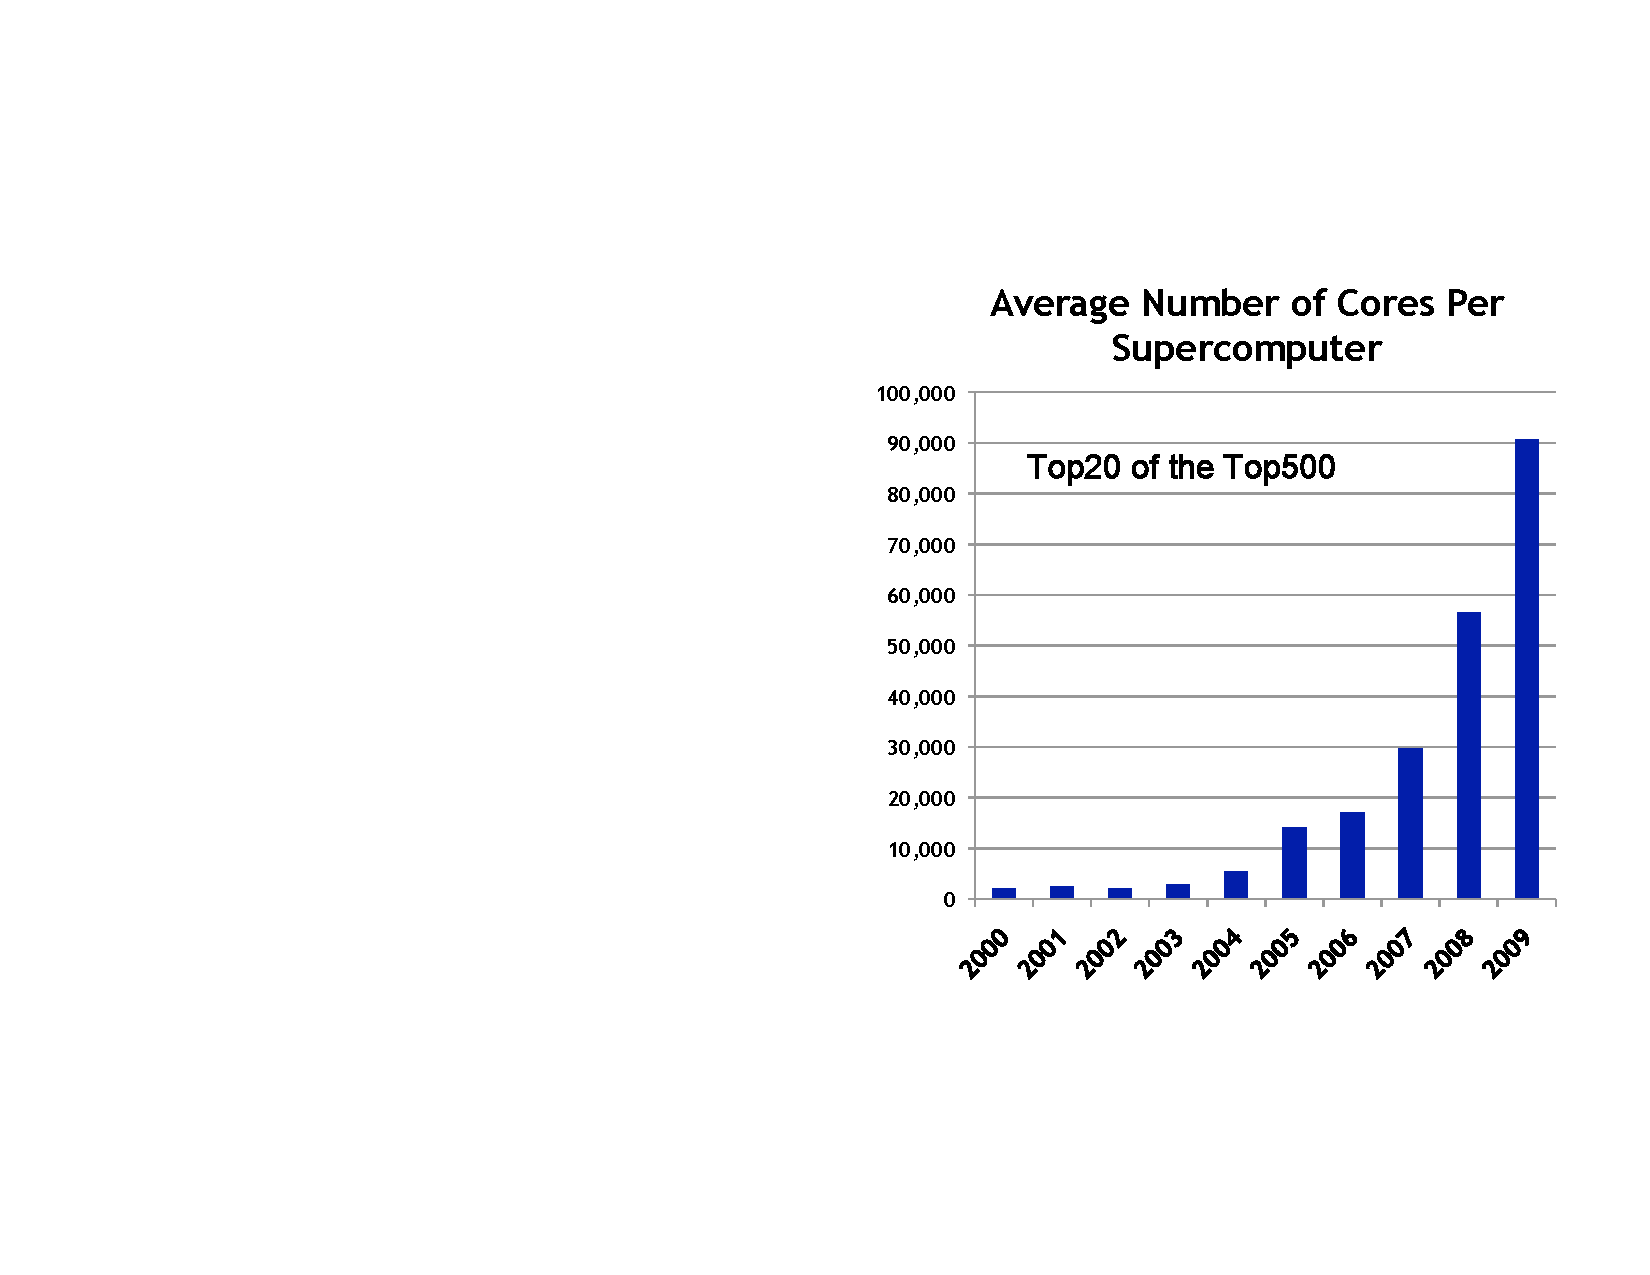
\includegraphics[width=0.48\textwidth]{hpc_cores.pdf}
        \caption{Average number of cores per supercomputer.}
        \label{fig:hpc_cores}
\end{figure}

\noindent
\textbf{How:}  소프트웨어 및 알고리즘 개발에 영향을 미칠 주요한 다섯가지 연구영역으로 나누어 기술변화를 예측하였다.
\bi
\ii 멀티코어 및 하이브리드 아키텍쳐에 맞게 소프트웨어 재설계 
\ii 자동 조정되는 응용 소프트웨어
\ii  성능을 위한 혼합 정밀도 활용하기
\ii 내고장성의 중요성
\ii 통신 회피 알고리즘
\ei

\noindent
\textbf{What:} Exascale computing으로 진화해 나가고 있는 HPC 하드웨어 및 소프트웨어 기술은 다음과 같다.
\bi
\ii Large-scale optics based interconnects
\ii Hardware and software based fault management
\ii Heterogeneous cores
\ii Another \textit{disruptive} technology
\bi
\ii Similar to what happened with \textit{cluster computing} and \textit{message passing}
\ei
\ei

\subsubsection{The Accelerated Cloud}
\textbf{Speaker:} Marc Hamilton\\
Vice President, Solutions Architecture and Engineering, NVIDIA, California, USA
\begin{figure}[htb]
        \centering
        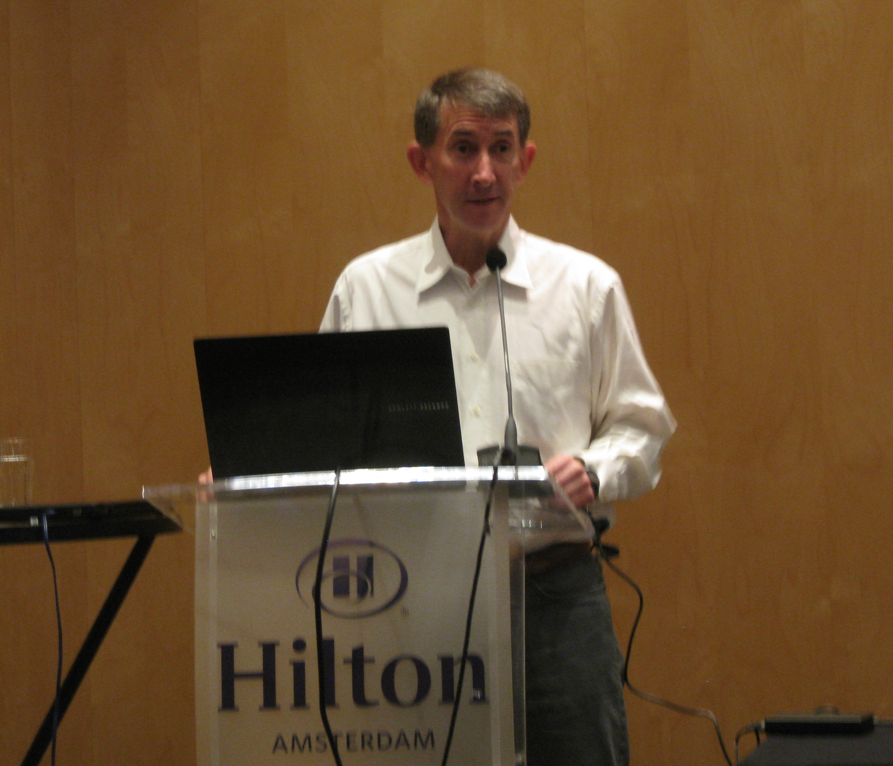
\includegraphics[width=0.45\textwidth]{marc.png}
        \caption{Marc Hamilton, NVIDIA}
        \label{fig:marc}
\end{figure}

\noindent
\textbf{Contributions:}  NVIDIA의 Marc Hamilton 기술이사 (그림 \ref{fig:marc})가 발표한 키노트는 
클라우드 컴퓨팅 및 HPC 기술 변화에 대해 살펴보고, NVIDIA의 GPU기반 클라우드 컴퓨팅 기술들에 대해 설명해 주었다. 
그림 \ref{fig:accelerated-data-center}은 GPU가 클라우드 컴퓨팅에 필요한 현재와 미래 유즈케이스를 보여 주고 있다.
구글은 공개적으로 내부 클라우드에 있는 GPU 1000대를 이용하여 40개의 GPU 가속 어플리케이션을 실행했다고 주장했다.
또한, 기계학습의 전문가인 Andrew Ng는 \textit{"향후 5년 내에, 50\%의 질의를 위해 사용되는 입력은 음성 또는 이미지다"} 라고 말했다.
이와 같이, GPU 기반 클라우드 컴퓨팅을 가속하기 위하여 NVIDIA는 주요 병목이였던 PCIe 버스 속도를 5배 개선한 NVLink 기술을 제공하고 있다고 한다.

\begin{figure}[htb]
        \centering
        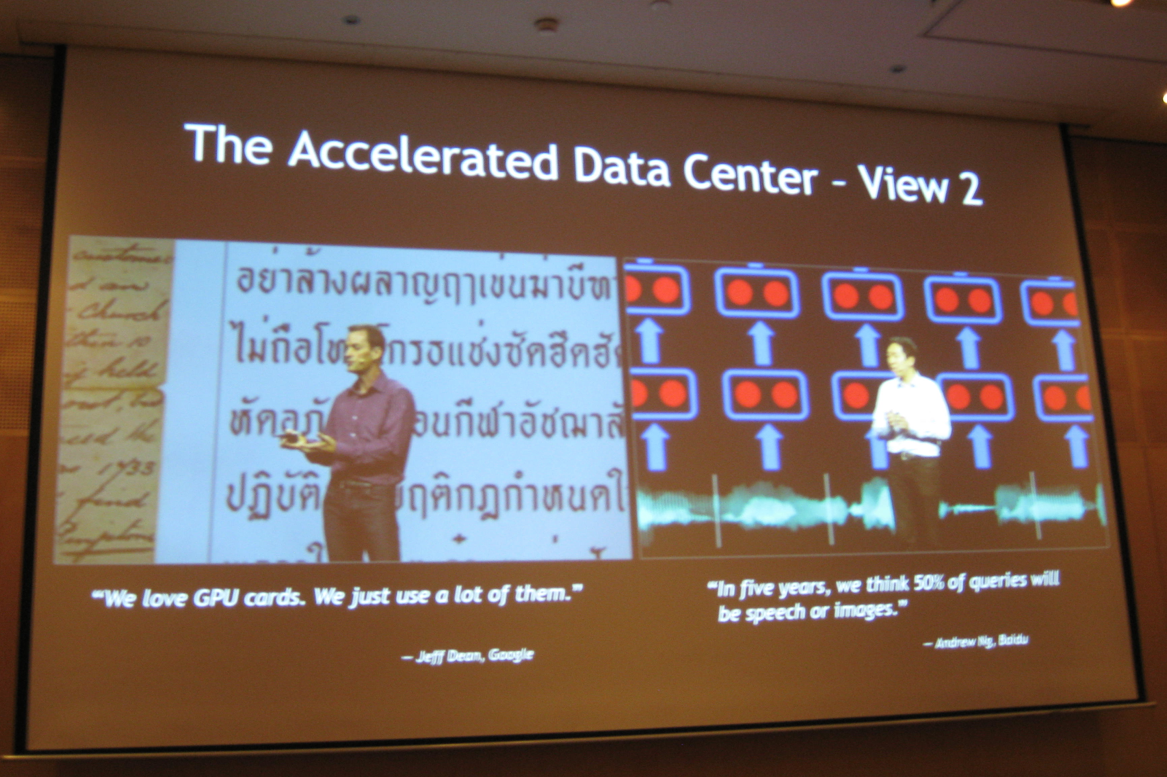
\includegraphics[width=0.48\textwidth]{marc-ppt.png}
        \caption{The Accelerated Data Center - View}
        \label{fig:accelerated-data-center}
\end{figure}

\noindent
\textbf{Technology Trends:}  가트너 (Gartner)의 서버 기술에 대한 2015년 하이퍼 사이클 \cite{George:2015}에 따르면, 신경망 실리콘 (\textit{Neural network silicon})이 대규모 데이터 병렬성을 가지는 문제를 해결하는 GPU 기반 하드웨어 가속화 기술이 이와 연관된다. 신경망 실리콘은 하이퍼 사이클상에서 현재(2015년 7월) 뜨는(on rise) 기술이며, 5년에서 10년사이에 정체기(plateau)에 접어들 것으로 가트너는 예상했다.
\begin{figure*}[htb]
        \centering
        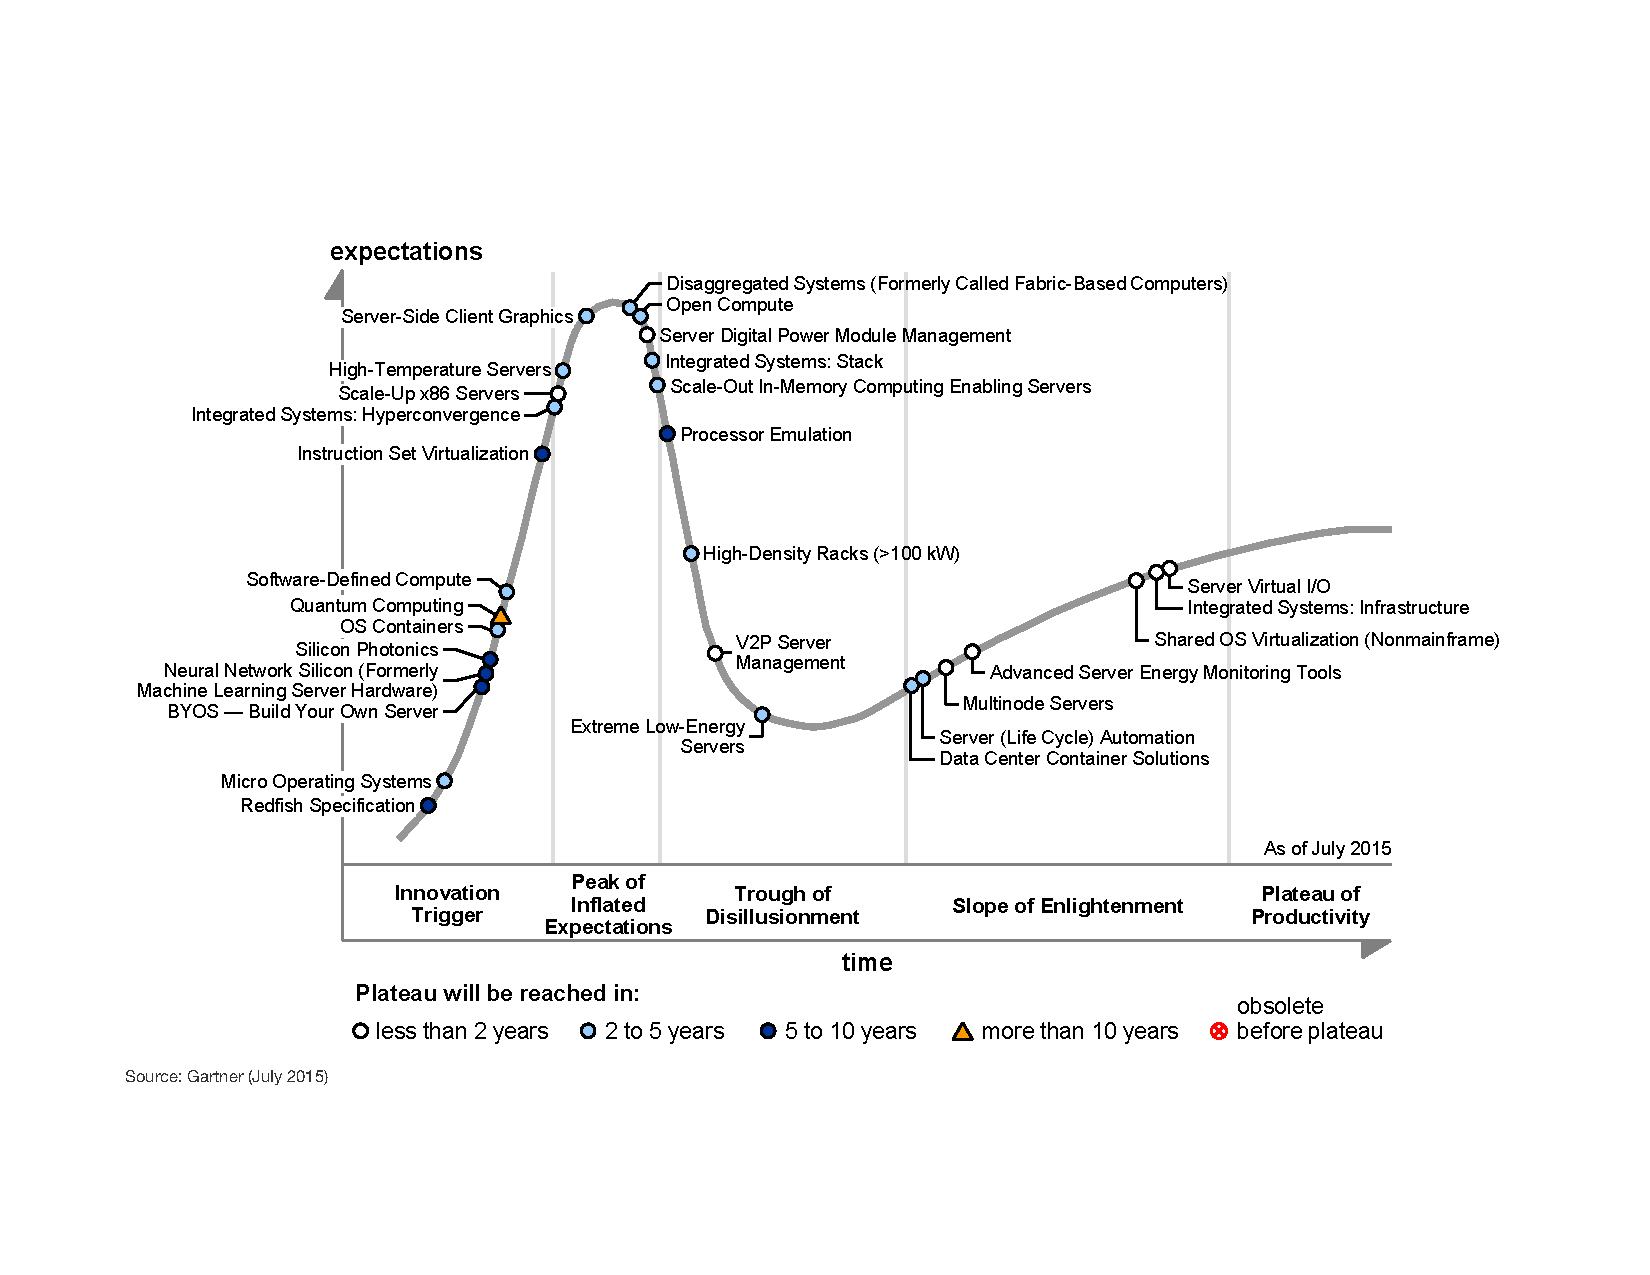
\includegraphics[width=1.0\textwidth]{gartner-server.pdf}
        \caption{Hype Cycle for Server Technologies, 2015 \cite{George:2015}}
        \label{fig:accelerated-data-center}
\end{figure*}
\bi
\ii \textbf{Neural Network Silicon:} 신경망 실리콘은 크게 깊은 신경망 (DNN; Deep Neural Network)을 이용한 기계학습 알고리즘의 성능을 향상 시킬수 있는 서버 기반 하드웨어 가속기를 의미한다. 
\ei

\noindent
\textbf{Note}  \textit{Deep Neural Networks}: 
"A \textit{deep neural network} (DNN) is an artificial neural network with multiple hidden layers of units between the input and output layers. DNNs can model complex nonlinear relationships. The extra layers enable composition of features from lower layers, giving the potential of modeling complex data with fewer units than a similarly performing shallow network." — From the Deep Neural Networks section of "Deep Learning", Wikipedia, 3 November 2014.

2012년 구글의 연구진은 DNN 기계학습 알고리즘을 GPU에 적용하여, 대규모 데이터 셋에 대한 학습시간(training time)을 획기적으로 단축시켰다고 한다.
또한, 모바일 장치 음성 인식과 웹 이미지 태깅에서 최근 개선들은 이러한 혁신과 직결된다고 볼 수 있다.

\noindent
\textbf{Why:}  전력 소비량은 HPC 시스템 운영에 있어서 중요한 이슈중에 하나다. 딥 러닝 (Deep learning)과 같은 대규모 데이터 병렬성이 요구되는 문제에는 GPU 하드웨어 자원을 이용하는 것이 전력 소비량에서 효과적이다. 다시 말해, GPU 기반 클라우드 컴퓨팅 및 데이터 센터는 수행 성능을 개선하면서 전력 소모 비용을 감축시킬 수 있는 방법이다.

\noindent
\textbf{How:}  NVIDIA는 GPU를 활용하여 데이터센터 및 클라우드 컴퓨팅의 성능 개선에 필요한 두가지 방법을 제공하고 있다.
첫 번째 방법은 기존의 CPU와 GPU사이의 PCIe 버스 병목을 해소하기 위한 방법으로 NVLink 기술을 제공한다.
두 번째 방법으로 CUDA 프로그래머를 위해 통합 메모리 (unified memory) 접근 기법과 고수준의 병렬 코드를 위한 프로그래밍 도구를 제공하는 것이다. 예를 들어,  동일한 C++ 코드를 NVIDIA GPU 코드, x86, ARM 그리고 Power CPU 코드로 변환 할 수 있는 Thrust 라이브러리를 제공한다.
이러한 두가지 방법을 지원하는 새로운 GPU 아키텍쳐인 파스칼 (Pascal) 아키텍쳐를 소개했다.

\begin{figure}[htb]
        \centering
        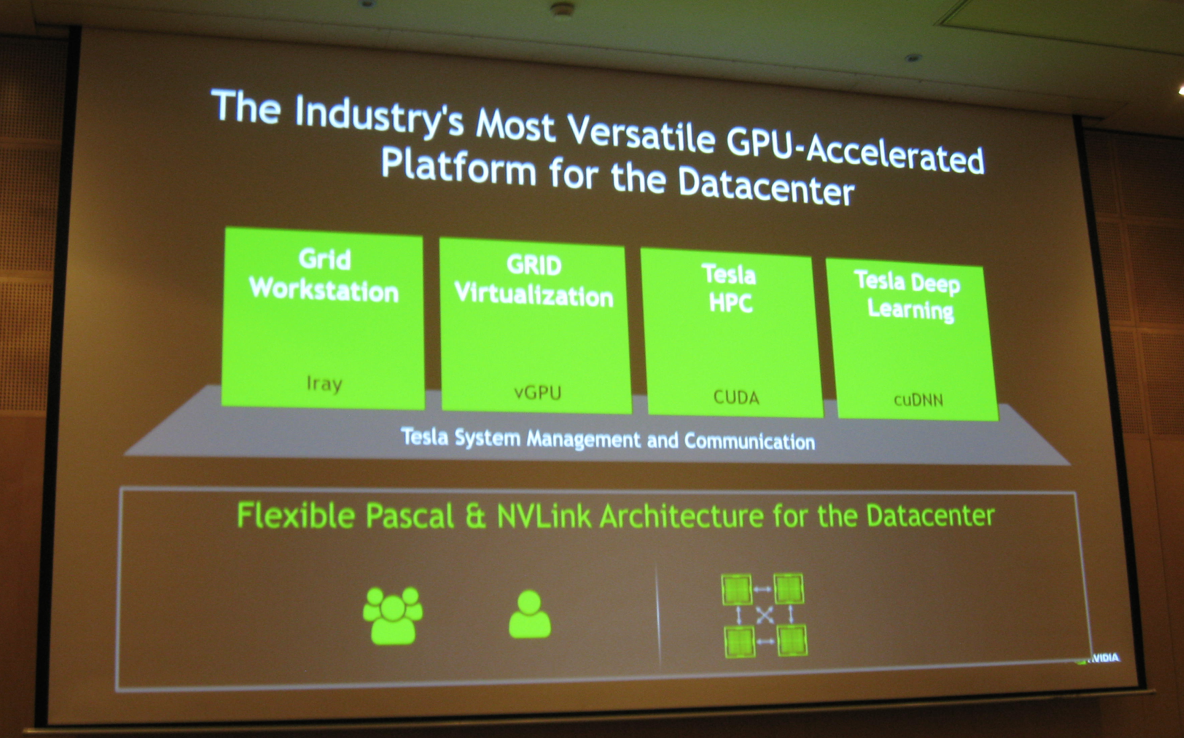
\includegraphics[width=0.48\textwidth]{gpu-platform.png}
        \caption{The industry's most versatile GPU-accelerated platform for the datacenter}
        \label{fig:gpu-accelerated-data-center}
\end{figure}

\noindent
\textbf{What:}  NVIDIA는 데이터 센터의 성능을 개선하기 위해 그림 \ref{fig:gpu-accelerated-data-center}과 같은 GPU 가속 기술을 적용한 플랫폼을 구축하여 운영하고 있다.
\bi
\ii Grid Workstation (Iray)
\ii GRID Virtualization (vGPU)
\ii Tesla HPC (CUDA)
\ii  Tesla Deep Learning (cuDNN)
\ii Tesla System Management and Communication
\ii  Flexible Pascal \& NVLink Architecture for the Datacenter: 파스칼 GPU는 170억개의 트랜지스터와 32GB VRAM을 갖추고 있다. (그림 \ref{fig:gpu-architecture})
\ei

\begin{figure}[htb]
        \centering
        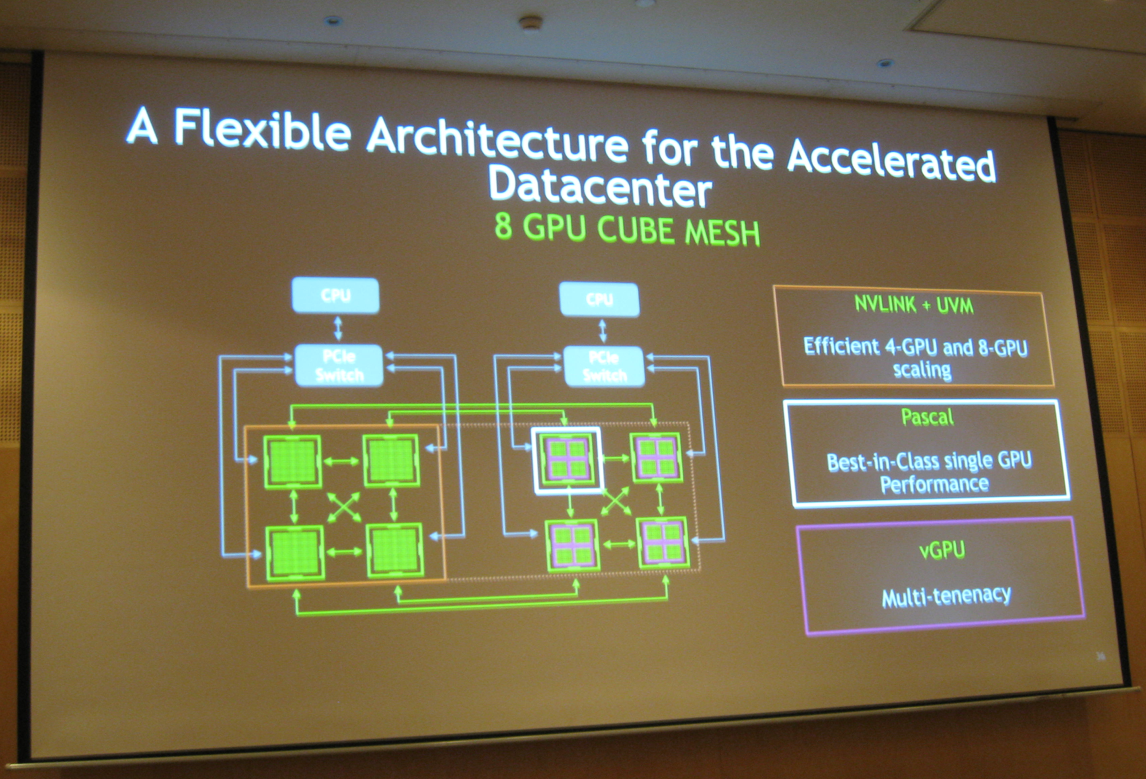
\includegraphics[width=0.48\textwidth]{gpu-architecture.png}
        \caption{A flexible architecture for the accelerated datacenter}
        \label{fig:gpu-architecture}
\end{figure}

\section{Paper Sessions}
\subsection{GENERAL PURPOSE GRAPHICS PROCESSING UNITS (GPGPU): : ACCELERATION, ALGORITHMS AND PERFORMANCE}

\subsubsection{A Runtime/Memory Trade-off of the Continous Ziggurat Method on GPUs}
\textbf{Speaker:} Christoph Riesinger (Technische Universitat Munchen, Munich, Germany)

\noindent
\textbf{Contributions:}  

\noindent
\textbf{Why:}  

\noindent
\textbf{How:}  

\noindent
\textbf{What:}  

\subsubsection{Cph CT Toolbox: A Performance Evaluation}
\textbf{Speaker:} Jonas Bardino (University of Copenhagen, Copenhagen, Denmark)

\noindent
\textbf{Contributions:}  

\noindent
\textbf{Why:}  

\noindent
\textbf{How:}  

\noindent
\textbf{What:}  

\subsubsection{Acceleration of dRMSD Calculation and Efficient Usage of GPU Caches}
\textbf{Speaker:} Jiri Filipovic (Masaryk University, Brno, Czech Republic)

\noindent
\textbf{Contributions:}  

\noindent
\textbf{Why:}  

\noindent
\textbf{How:}  

\noindent
\textbf{What:}  

\subsubsection{Optimizing Communications in multi-GPU Lattice Boltzmann Simulations}
\textbf{Speaker:} Sebastiano Fabio Schifano (Universita di Ferrara and INFN, Ferrara, Italy)

\noindent
\textbf{Contributions:}  

\noindent
\textbf{Why:}  

\noindent
\textbf{How:}  

\noindent
\textbf{What:}  

\subsection{HIGH PERFORMANCE MEMORY SYSTEMS AND DISTRIBUTED STORAGE AND WAREHOUSING}
\subsubsection{Analysis of Asymmetric 3D DRAM Architecture in Combination with L2 Cache Size Reduction}
\textbf{Speaker:} Alex Schoenberger (Technische Universität Darmstadt, Darmstadt, Germany)
\noindent
\textbf{Contributions:}  

\noindent
\textbf{Why:}  

\noindent
\textbf{How:}  

\noindent
\textbf{What:}  

\subsubsection{Tracing Long Running Applications: A Case Study Using Gromacs}
\textbf{Speaker:} Michael Wagner (Center for Information Services and High Performance Computing (ZIH), Technische Universitat Dresden, Dresden, Germany)
\subsubsection{Advanced Commands and Distributed Data Layout to Enhance the SSD Internal Parallelism}
\textbf{Speaker:} Soraya Zertal (PRiSM, Université de Versailles, Versailles, France)
\noindent
\textbf{Contributions:}  

\noindent
\textbf{Why:}  

\noindent
\textbf{How:}  

\noindent
\textbf{What:}  

\subsection{HPCS 2015 POSTER PAPERS}
호텔 로비에서 포스터 세션이 진행되었고, 포스터 논문은 아래 6개의 논문이 발표되었다.  
\be
\ii Real-time Signal Identification in Big Data Streams Bragg–Spot Localization in Photon Science
\ii A Resilient Routing Approach for Mobil Ad Hoc Networks
\ii Efficient Asian Option Pricing with CUDA
\ii GPGPU Performance Evaluation of Some Basic Molecular Dynamics Algorithms
\ii Cookery: A Framework for Developing Cloud Applications
\ii Subordination: Cluster Management without Distributed Consensus
\ee

\begin{figure}[htb]
        \centering
        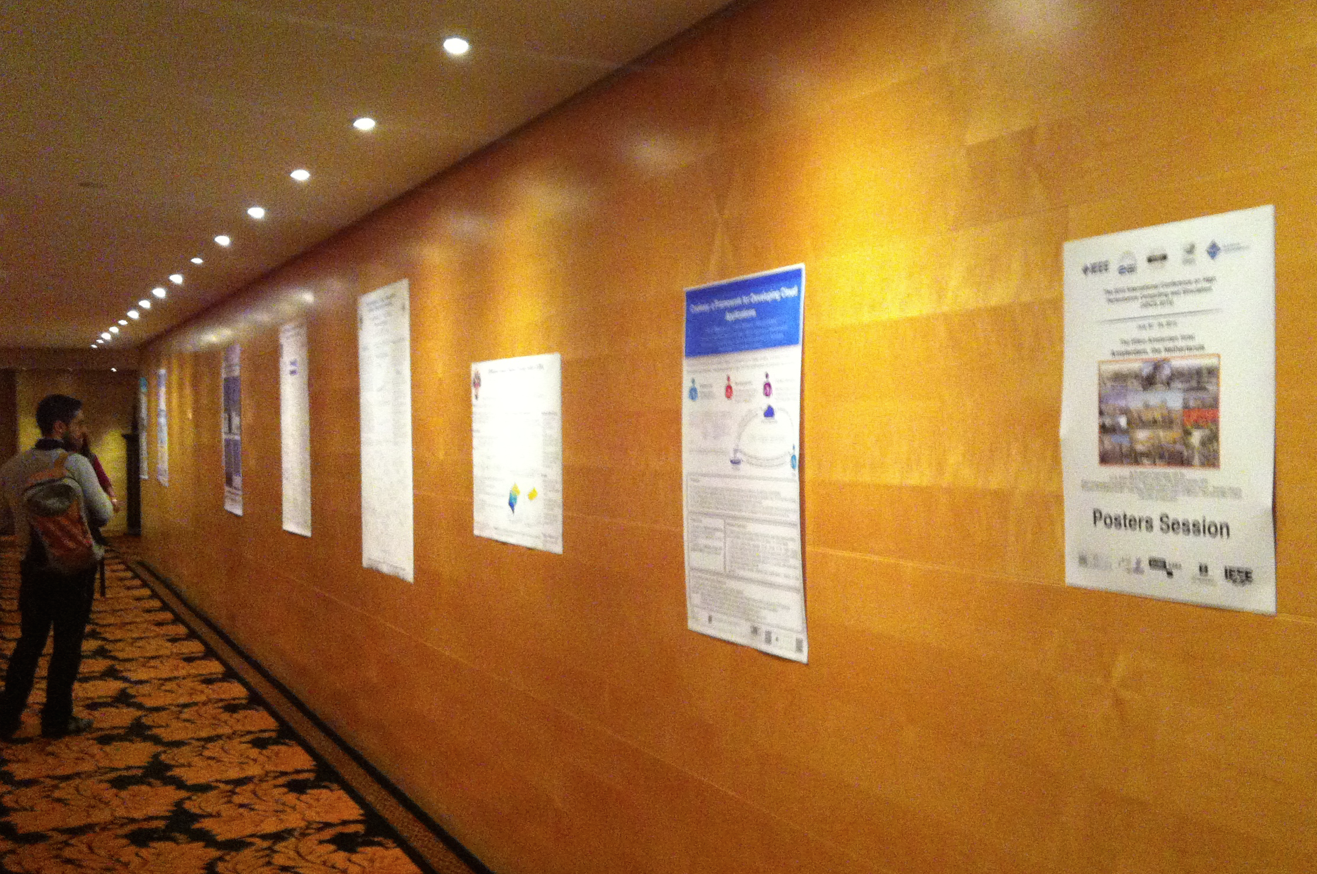
\includegraphics[width=0.48\textwidth]{posters.png}
        \caption{HPCS 2015 Poster Papers}
        \label{fig:posters}
\end{figure}

\subsection{HIGH PERFORMANCE MOBILE ARCHITECTURES, WIRELESS NETWORKS AND APPLICATIONS}
\subsubsection{GPU Accelerated Ray Launching for High-Fidelity Virtual Test Drives of VANET Applications}
\textbf{Speaker:} Manuel Schiller, (Lehrstuhl fur Echtzeitsysteme und Robotik, Technische Universitat Munchen, Germany)
\noindent
\textbf{Contributions:}  

\noindent
\textbf{Why:}  

\noindent
\textbf{How:}  

\noindent
\textbf{What:}  

\subsubsection{A Collaboration Middleware for Service Scalability in Peer-to-Peer Systems}
\textbf{Speaker:} Sung-Soo Kim (ETRI, Daejeon, South Korea)

필자가 발표한 논문으로 피어투피어 시스템에서 다양한 응용 어플리케이션간의 협업을 지원할 수 있는 미들웨어에 대해 발표했다.
발표 후, 아래와 같이 2가지 질문이 있었다.

\bi
\ii \textbf{Question 1:} 미들웨어에서 관리하고 있는 논리적 앱 라이프 사이클이 안드로이드의 Activity 라이프 사이클과는 어떻게 다른가?\\
\textbf{Answer 1:} 논리적 앱 라이프 사이클은 동일 네트워크에 있는 모든 디바이스들이 함께 공유하는 것이다. 하지만, 안드로이드 액티비티 라이프 사이클은 각각의 디바이스에서 독립적으로 관리된다. 논리적 앱에서 앱이 특정 디바이스에서 다른 디바이스로의 이주 (Migration)를 하는 경우, 이주에 대한 라이프 사이클 상태가 있다. 하지만, 안드로이드 액티비티 라이프 사이클에는 단일 디바이스에 대한 상태이므로, 이주 (Migration) 상태가 없다.
\ii \textbf{Question 2:} 앱간 연관성 정보 및 앱간 메세지 정보에 대한 보안은 어떻게 처리했는가?\\
\textbf{Answer 1:} 메세지 암호화 및 정보 보안에 관련된 내용은 현재 구현되어 있지 않지만, 향후 연구로 계획되어 있다. 메세지 암호화는 AES (Advanced Encryption System)을 적용하여 구현할 예정이다.
\ei

\noindent
\textbf{Contributions:} 피어투피어 시스템에 존재하는 멀티스크린 디바이스의 앱관 연관성, 콘텐츠간 연관성 스키마 정의언어를 이용하여, 협업을 제공하는 서비스를 구성할 수 있으며, 대칭형 협업 (symmetric collaboration)을 제공하는 최초의 미들웨어를 설계/구현하였다. 그림 \ref{fig:middleware-architecture}d은 우리 논문에서 제안한 협업미들웨어 구조와 서비스 플랫폼 구조를 보여주고 있다.

\begin{figure}[htb]
        \centering
        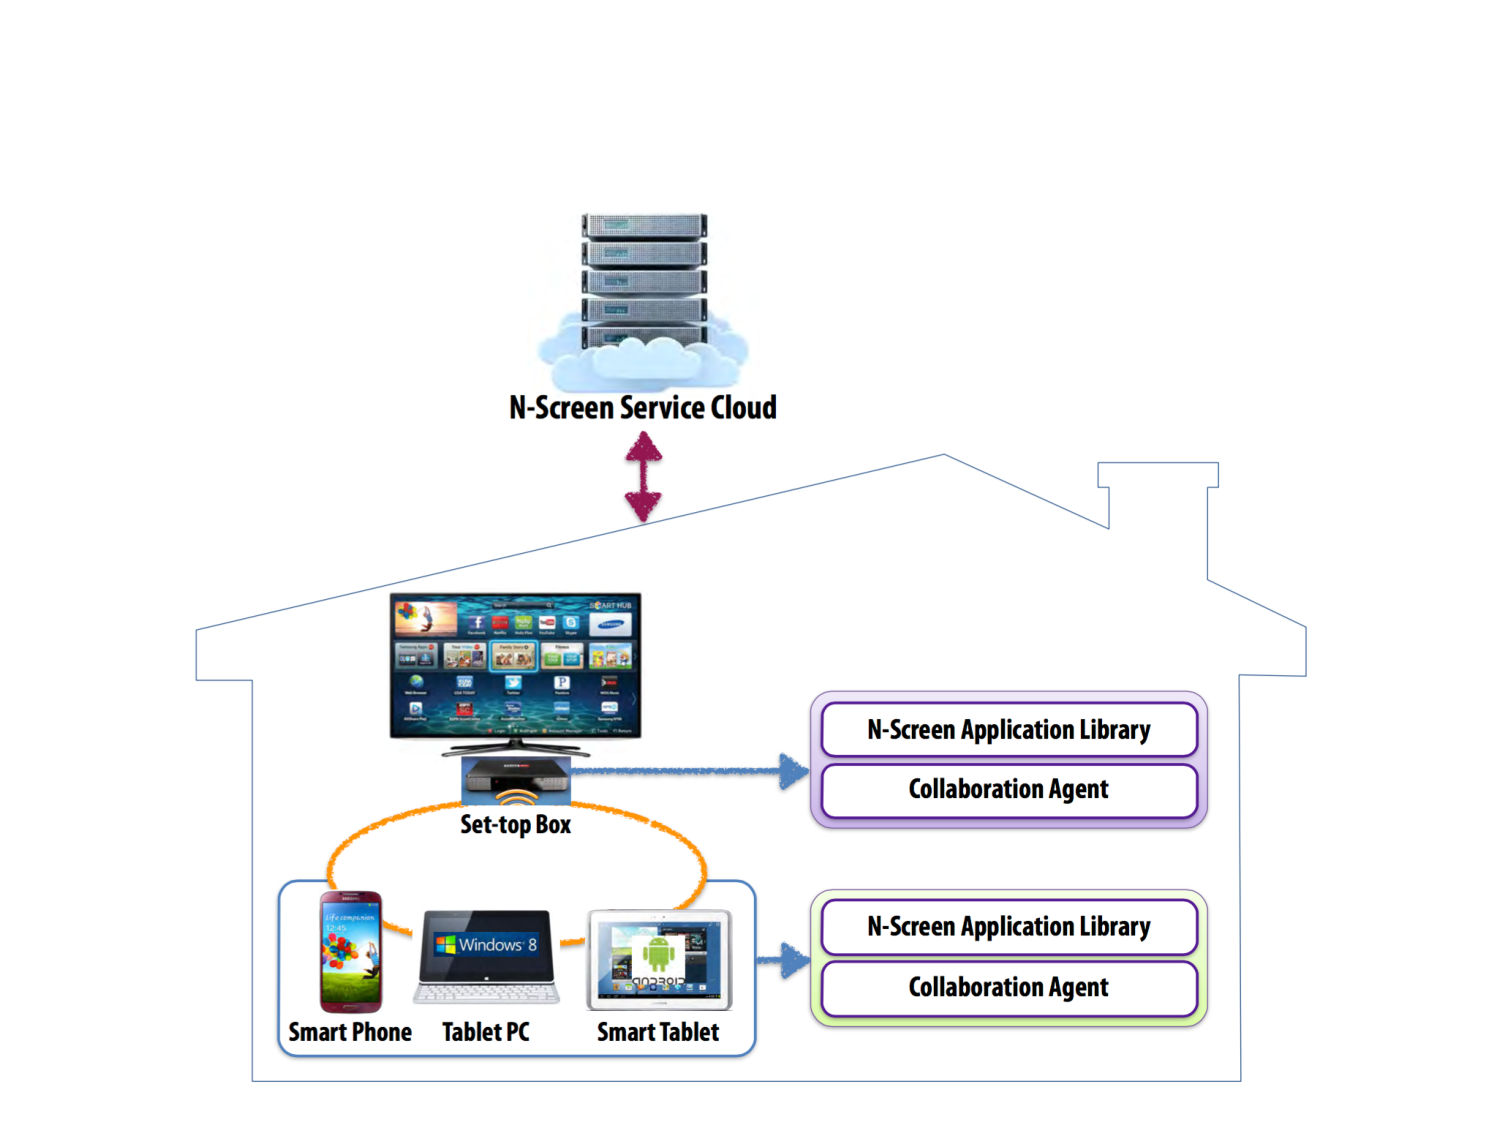
\includegraphics[width=0.48\textwidth]{middleware.pdf}
        \caption{A architecture for the collaboration middleware}
        \label{fig:middleware-architecture}
\end{figure}

\noindent
\textbf{Why:} 기존 스마트 디바이스간 협업을 위해서는 특정 디바이스(예; 스마트 TV)를 중심으로 한 마스터 슬레이브 형태의 계층적 협업만을 제공할 수 있었다. 스마트 디바이스가 각각이 동등한 역할로 피어투피어 형태의 대칭협 협업과 서비스 확장성을 제공하는 것이 중요하다. 

\noindent
\textbf{How:}  논문의 협업 미들웨어는 세가지 구성요소인 서비스 개발자를 위한 N-스크린 어플리케이션 라이브러리, 최종 사용자를 위한 협업 위젯, 그리고 각 스마트 디바이스에 설치되는 협업 에이전트를 포함하고 있다. 미들웨어는 협업 기반의 N-스크린 서비스를 개발에 필요한 공통적인 기능들; 스마트 디바이스 관리, 응용프로그램 및 컨텍스트 관리, 협업세션 관리, 앱 생명주기 관리 등의 기능을 제공한다.

\noindent
\textbf{What:} 미들웨어는 크게 두가지 계층으로 나누어 진다. 서비스 개발자가 새로운 서비스 개발을 위한 N-스크린 어플리케이션 라이브러리 (NSAL)과 디바이스 협업 미들웨어를 설계하고 개발했다. 각 디바이스의 어플리케이션 및 어플리케이션 컨텍스트 정보는 N-스크린 클라우드 서버가 관리한다. 본 연구의 주요 산출물은 아래와 같다.
\bi
\ii N-Screen Service Cloud
\ii N-Screen Application Library
\ii Collaboration Agent
\ei

\subsubsection{Experiments in Fair Scheduling in 4G WiMAX and LTE}
\textbf{Speaker:} Junaid Ahmed Zubairi (State University of New York at Fredonia, New York, USA)
\noindent
\textbf{Contributions:}  

\noindent
\textbf{Why:}  

\noindent
\textbf{How:}  

\noindent
\textbf{What:}  

\subsection{IMAGE PROCESSING, MACHINE LEARNING, PATTERN RECOGNITION \& APPLICATIONS}
\subsubsection{A Reduced Complexity Instruction Set Architecture for Low Cost Embedded Processors}
\textbf{Speaker:} Mabo Ito (The University of British Columbia - Vancouver, British Columbia, Canada)
\noindent
\textbf{Contributions:}  

\noindent
\textbf{Why:}  

\noindent
\textbf{How:}  

\noindent
\textbf{What:}  

\subsubsection{Deep Learning with Shallow Architecture for Image Classification}
\textbf{Speaker:} Asma ElAdel (National School of Engineers of Sfax, Sfax, Tunisia)
\noindent
\textbf{Contributions:}  

\noindent
\textbf{Why:}  

\noindent
\textbf{How:}  

\noindent
\textbf{What:}  

\subsubsection{An Efficient Implementation of Fuzzy Edge Detection Using GPUs in MATLAB}
\textbf{Speaker:} Farnaz Hoseini (Islamic Azad University, Rasht, Iran; University of Guilan, Rasht, Iran)
\noindent
\textbf{Contributions:}  

\noindent
\textbf{Why:}  

\noindent
\textbf{How:}  

\noindent
\textbf{What:}  

\subsection{RESOURCE ALLOCATION, SCHEDULING, AND LOAD BALANCING IN HPC SYSTEMS}
\subsubsection{Market-inspired Dynamic Resource Allocation in Many-core High Performance Computing Systems}
\textbf{Speaker:} Amit Kumar Singh (University of York, York, U.K.)
\noindent
\textbf{Contributions:}  

\noindent
\textbf{Why:}  

\noindent
\textbf{How:}  

\noindent
\textbf{What:}  

\subsubsection{234 Scheduling of 3-2 and 2-1 Eliminations for Parallel Image Compositing using Non-Power-of-Two Number of Processes}
\textbf{Speaker:} Jorji Nonaka (RIKEN Advanced Institute of Computational Science, Kobe, Japan; Light Transport Entertainment, Inc., Tokyo, Japan)
\noindent
\textbf{Contributions:}  

\noindent
\textbf{Why:}  

\noindent
\textbf{How:}  

\noindent
\textbf{What:}  

\subsubsection{In Search of the Best MPI-OpenMP Distribution for Optimum Intel-MIC Cluster Performance}
\textbf{Speaker:} Gladys Utrera (Universitat Politecnica de Catalunya-Barcelona, Barcelona, Spain)
\noindent
\textbf{Contributions:}  

\noindent
\textbf{Why:}  

\noindent
\textbf{How:}  

\noindent
\textbf{What:}  

% Example Figure
%%%%%%%%%%%%%
%\begin{figure}[htb]
%        \centering
%        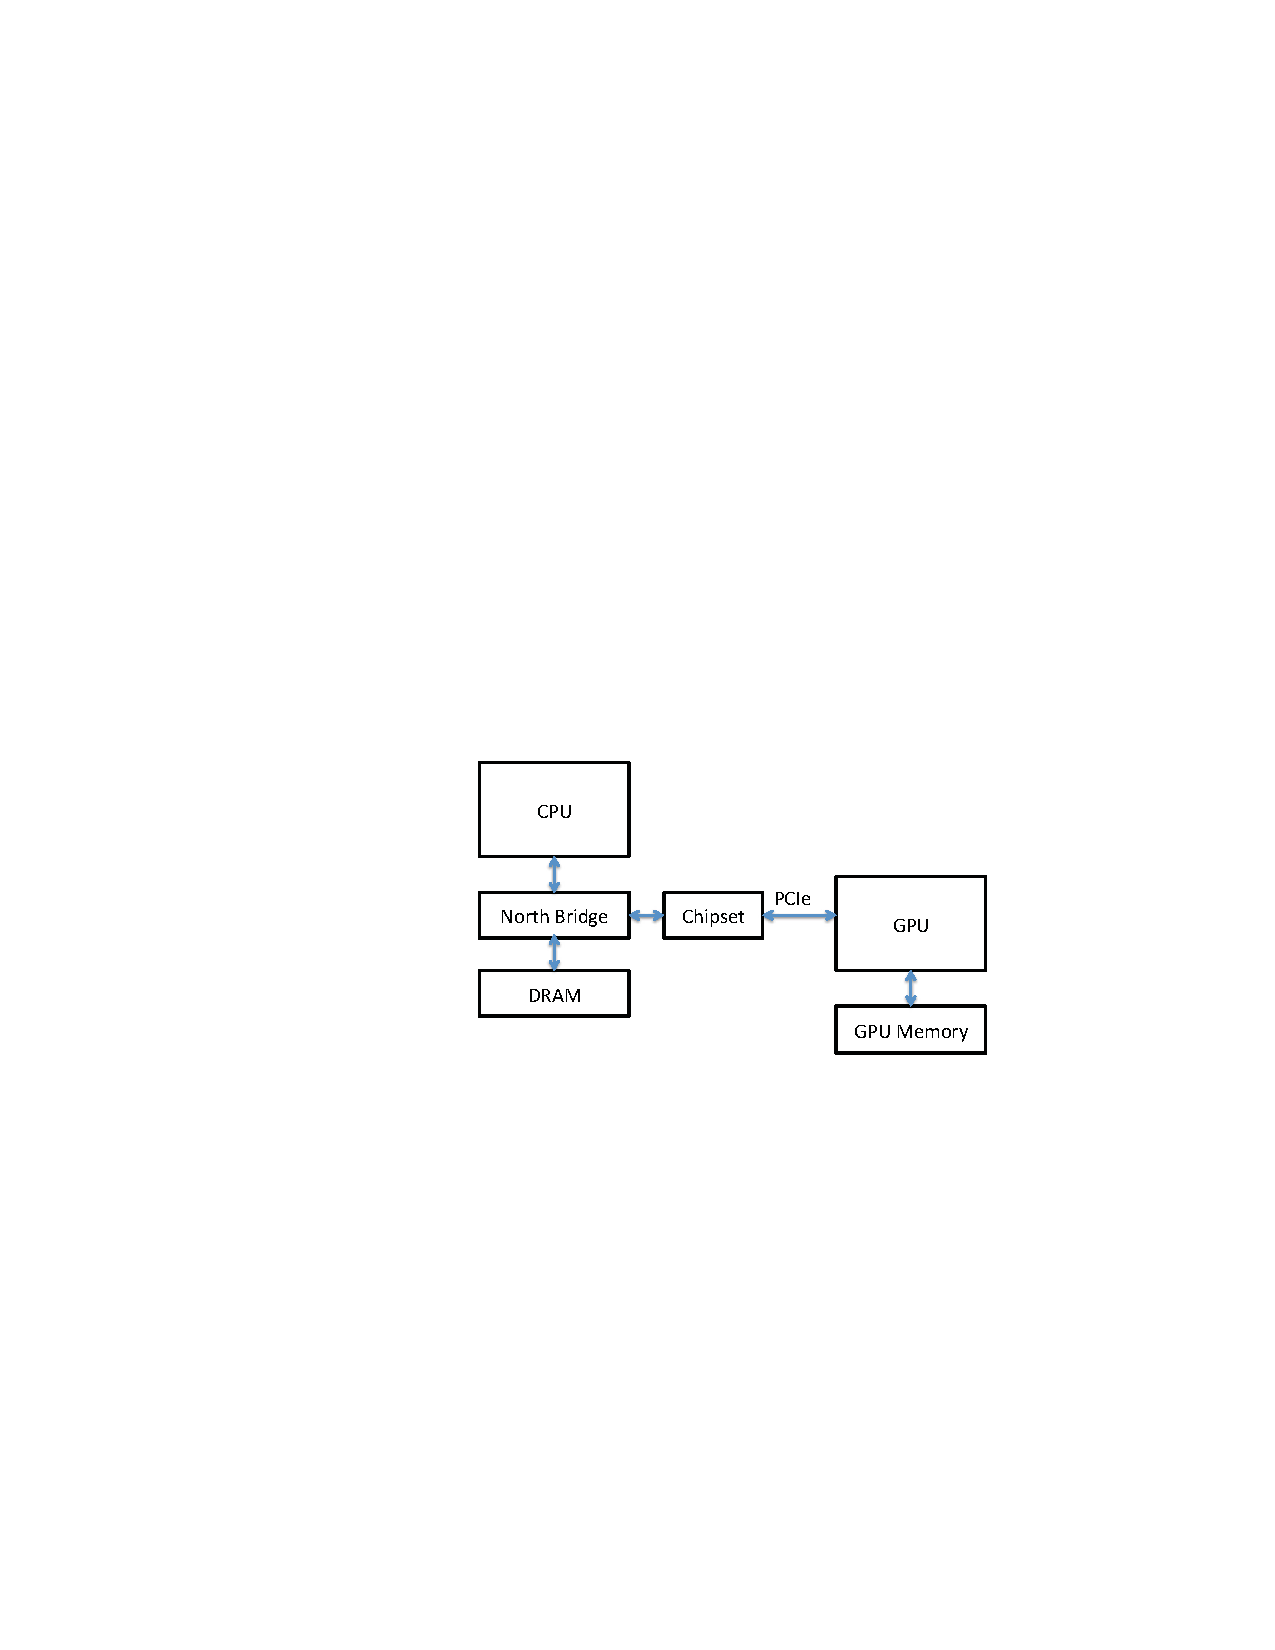
\includegraphics[width=0.48\textwidth]{system-overview.pdf}
%        \caption{A system overview with CPU and a discrete GPU.}
%        \label{fig:system_overview}
%\end{figure}


\section{만난 사람들}

\begin{figure}[htb]
        \centering
        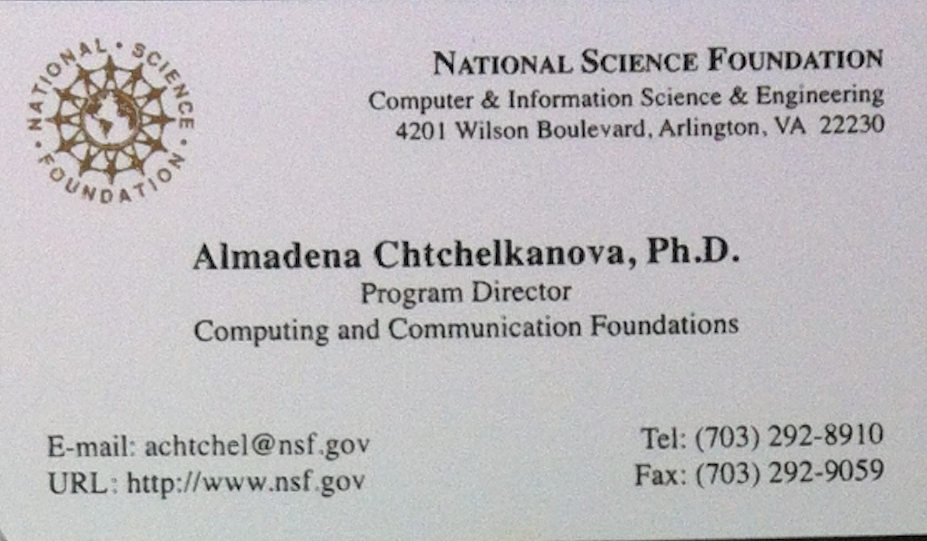
\includegraphics[width=0.48\textwidth]{nc01.png}
        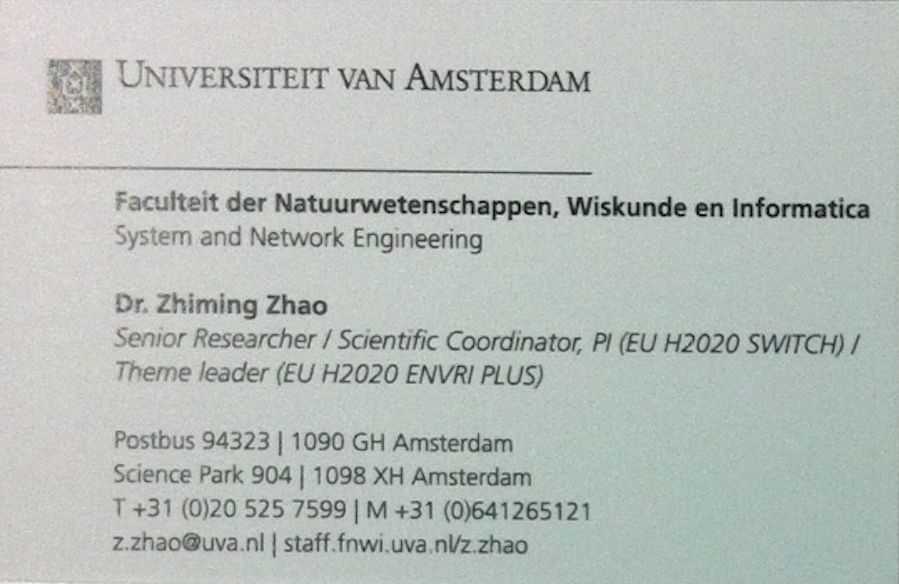
\includegraphics[width=0.48\textwidth]{nc02.png}
        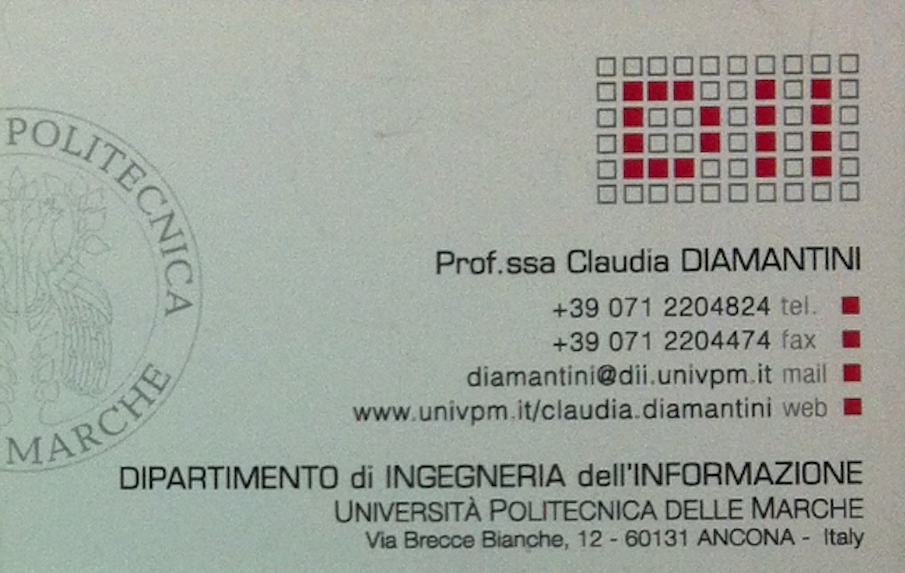
\includegraphics[width=0.48\textwidth]{nc03.png}
        \caption{교류한 연구자 명함}
        \label{fig:namecards01}
\end{figure}

\begin{figure}[htb]
        \centering
        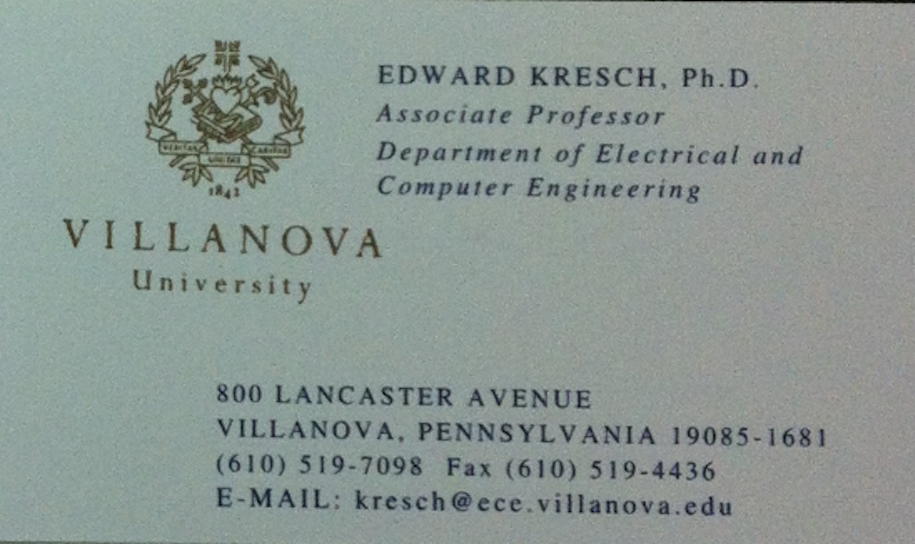
\includegraphics[width=0.48\textwidth]{nc04.png}
        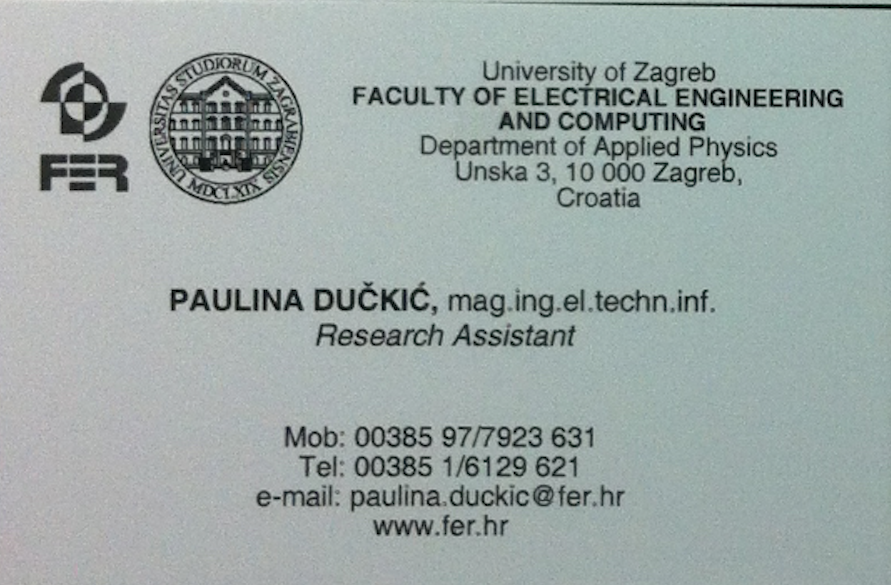
\includegraphics[width=0.48\textwidth]{nc05.png}
        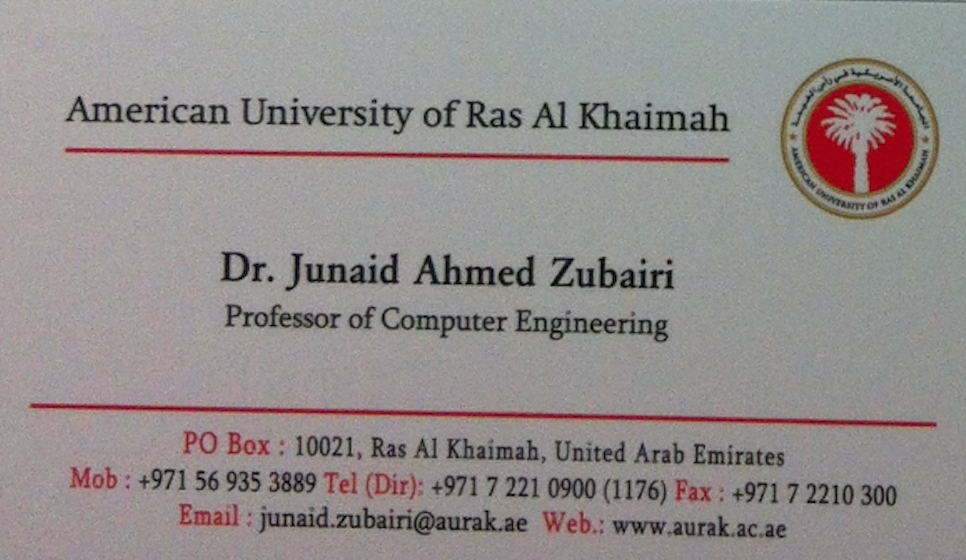
\includegraphics[width=0.48\textwidth]{nc06.png}
        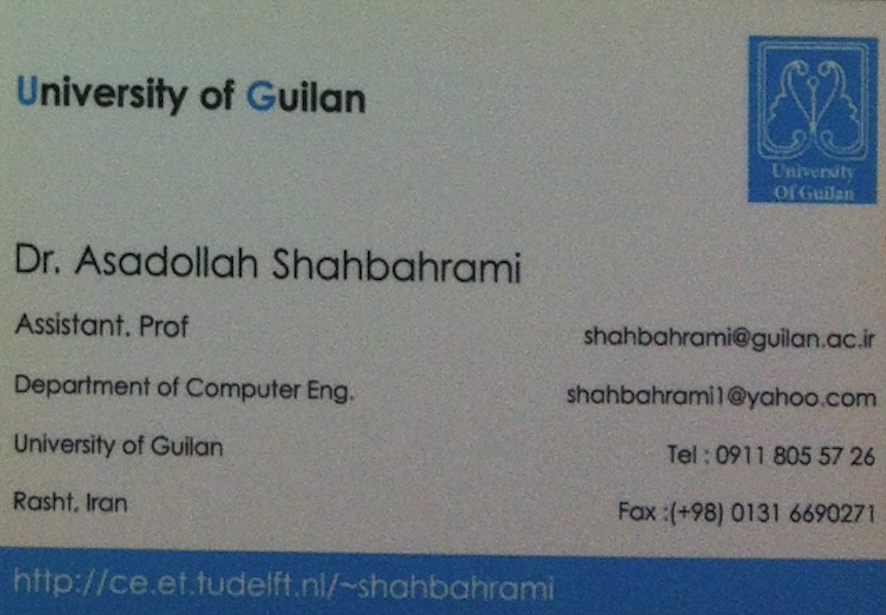
\includegraphics[width=0.48\textwidth]{nc07.png}
        \caption{교류한 연구자 명함}
        \label{fig:namecards02}
\end{figure}

\section{암스테르담 숙소 및 교통정보}

\section{결론}



\bibliographystyle{abbrv}
\bibliography{sqlonhadoop}

\end{document}
